\documentclass[8pt]{beamer}
\usepackage[utf8]{inputenc}
\usepackage{graphicx}
\usepackage{caption}
\usepackage{blindtext}
\usepackage{url}
\usepackage{tikz}
\usetikzlibrary{arrows}
\usetikzlibrary{arrows.meta,positioning}
\tikzset{>=latex} % for LaTeX arrow head
\usetikzlibrary{shapes.geometric}
\usepackage{derivative}
\usepackage{svg}
\usepackage{adjustbox}
\usepackage{etoolbox}

\usetheme{Darmstadt}
\usecolortheme{default}

\usepackage[bibstyle=ieee, citestyle=numeric-comp, url=false]{biblatex}
\addbibresource{references.bib}

\setbeamertemplate{caption}[numbered]
\setbeamertemplate{bibliography item}{\insertbiblabel}

\def\signed #1{{\leavevmode\unskip\nobreak\hfil\penalty50\hskip1em
  \hbox{}\nobreak\hfill #1%
  \parfillskip=0pt \finalhyphendemerits=0 \endgraf}}

\newsavebox\mybox
\newenvironment{aquote}[1]
  {\savebox\mybox{#1}\begin{quote}}
  {\vspace*{1mm}\signed{\usebox\mybox}\end{quote}}

\usepackage{derivative}
\usepackage{subcaption}
\usepackage{color}
\pgfdeclarelayer{back} % to draw on background
\pgfsetlayers{back,main} % set order
\usepackage{ifthen}
\usetikzlibrary{shapes.geometric}
\definecolor{s-color}{HTML}{41949A}
\definecolor{i-color}{HTML}{E56E5A}
\definecolor{r-color}{HTML}{7384BB}
\renewcommand\thesubfigure{\roman{subfigure}}

\renewcommand*{\bibfont}{\small}

%------------------------------------------------------------
%This block of code defines the information to appear in the
%Title page
\title{\Large Simulating the Effects of Risk Perception and Human Behaviour on a Vector-borne Disease with Agent-based Modelling}

\subtitle{\normalsize MCS Oral Presentation}

\author{Jack Oliver (1389498)}

\institute
{\normalsize
  % \inst{1}%
  \textbf{Primary Supervisor}\\
  Associate Professor Nic Geard
  \and
  % \inst{2}%
  \textbf{Co-Supervisor}\\
  Dr Cameron Zachreson
}

\date{}
% \date[VLC 2021] % (optional)
% {Very Large Conference, April 2021}

%End of title page configuration block
%------------------------------------------------------------



%------------------------------------------------------------
%The next block of commands puts the table of contents at the 
%beginning of each section and highlights the current section:

% \AtBeginSection[]
% {
%   \begin{frame}
%     \frametitle{Table of Contents}
%     \tableofcontents[currentsection]
%   \end{frame}
% }
%------------------------------------------------------------


\begin{document}

\captionsetup[figure]{font=footnotesize, labelfont=bf, labelsep=period}
\newcommand{\bcaption}[2]{\caption{\textbf{#1} #2}}

%The next statement creates the title page.
\frame{\titlepage}


%---------------------------------------------------------
%This block of code is for the table of contents after
%the title page
% \begin{frame}
% \frametitle{Table of Contents}
% \tableofcontents
% \end{frame}
%---------------------------------------------------------


\section{Background and motivation}

%---------------------------------------------------------
%Changing visivility of the text
\begin{frame}
\frametitle{Preventive behaviour: a shared example}

\begin{columns}[t!]
    \begin{column}{4cm}
        \begin{figure}
            \centering
            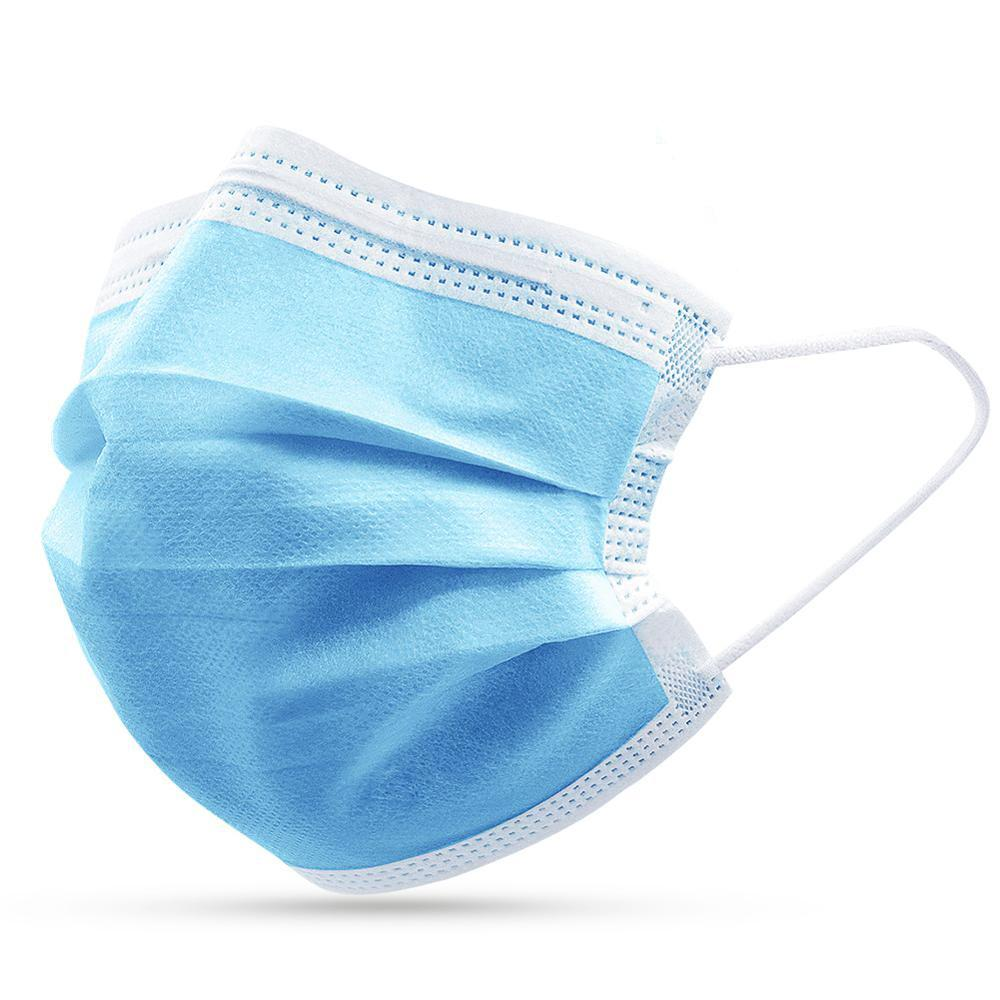
\includegraphics[width=4cm]{img/face_mask.jpg}
            \caption*{\footnotesize Source: SCIG\footnotemark[1]}
        \end{figure}
    \end{column}

    \begin{column}{6cm}
    \begin{itemize}
        \setlength\itemsep{.5cm}
        \item Think of a time when you wore---or didn't wear---a face mask (when masks weren't mandated). \pause
        \item What motivated you to protect (or not protect) yourself? \pause
        \item Was it because\dots
        \begin{itemize}
            \item you felt like you might get infected? \pause
            \item you thought you might infect others? \pause
            \item you were used to wearing one? \pause
            \item you just wanted to fit in?
        \end{itemize}
            
    \end{itemize}
    \end{column}
\end{columns}

\pause
% \begin{aquote}{\textcite{tan_severe_2004}}
%     ``[W]hen people perceive a health problem as serious they will take some kind of action.''
% \end{aquote}
\vspace{.5cm}
\textbf{Preventive behaviours} (the use of preventive measures) differ among individuals because of unique thought processes and varying motivating factors for protection.

\footnotetext[1]{\scriptsize \url{https://southerncrossgroup.com.au/product/disposable-medical-face-mask/}\vspace{.2cm}}

\end{frame}

%---------------------------------------------------------

\subsection{Epidemiological background}

%---------------------------------------------------------
%Changing visivility of the text
\begin{frame}
\frametitle{Vector-borne diseases}

\begin{columns}[t!]
    \begin{column}{5cm}
        \begin{figure}
            \centering
            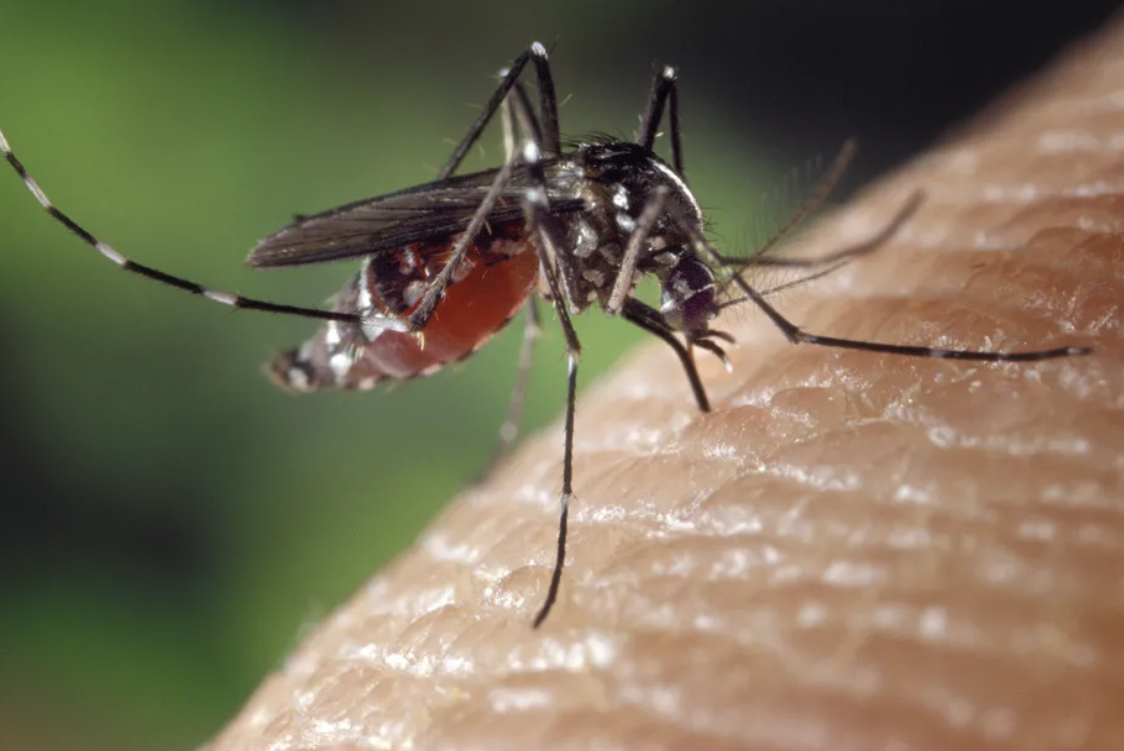
\includegraphics[width=5cm]{img/mosquito}
            \caption*{\footnotesize Source: James Gathany/CDC\footnotemark[1]}
        \end{figure}
    \end{column}

    \begin{column}{5cm}
    \begin{itemize}
        \item E.g. malaria, dengue, chikungunya, leishmaniasis.
        \item $\mathbf{\ge}$ 700,000 deaths annually.
        \item Account for more than 17\% of all infectious diseases \cite{world_health_organisation_who_vector-borne_2020}.
    \end{itemize}
    \end{column}
\end{columns}

\vspace{.25cm}
\begin{itemize}
    \item Community-based interventions
    \begin{itemize}
        \item Chemical: insecticides, coils
        \item Non-chemical: long-sleeved clothing, staying indoors
    \end{itemize}
\end{itemize}

\vspace{.5cm}
\textbf{There is a need to better understand the dynamics between vector-borne diseases and preventive behaviours to design effective community-based interventions.}
% \textbf{How can we design better community-based interventions by understanding the dynamics between vector-borne diseases and preventive behaviours?}

\vspace{.5cm}
\footnotetext[1]{\scriptsize \url{http://phil.cdc.gov/phil/details.asp?pid=1969}}

\end{frame}

%---------------------------------------------------------


%---------------------------------------------------------
% \begin{frame}
% \frametitle{Risk perception and behaviour}

% \begin{aquote}{\textcite{tan_severe_2004}}
%     ``[W]hen people perceive a health problem as serious they will take some kind of action.''
% \end{aquote}.

% \begin{itemize}
%     \item In order to adopt preventive measures, individuals must have a \textbf{sufficiently high risk perception} of a disease.
%     \item Because CBIs are a \textit{bottom-up} approach to tackling VBDs, they \textbf{must influence individuals' risk perception and behavioural attitudes} towards preventive measures.
%     \item While many \alert{psychological models for why people change their behaviour} exist, the area remains understudied, especially in the context of CBIs and VBDs.
% \end{itemize}

% \vspace{.5cm}
% Policymakers need to understand the interactions between disease spread, risk perception, and \textit{preventive behaviours}---behaviours that involve the use of preventive measures.

% \end{frame}
%---------------------------------------------------------

\subsection{Modelling approaches}


%---------------------------------------------------------
% \begin{frame}
% \frametitle{Mathematical models for disease spread}

% Traditional models of VBD spread have historically paid little attention to the behaviour of individuals.
% %You may be familiar with the \textit{SIR} (Susceptible, Infected, and Recovered) model:

% \begin{figure}
     \centering
     \begin{subfigure}[b]{0.3\textwidth}
         \centering
         \begin{align*}
             \odv{S}{t} &= -\beta S I \\[.15cm]
             \odv{I}{t} &=\beta S I - \gamma I \\[.15cm]
             \odv{R}{t} &=\gamma I
         \end{align*}
         % \vspace{.5cm}
         % \caption{}
         \label{fig:sir-eqs}
     \end{subfigure}%
     \hfill
     \begin{subfigure}[b]{0.3\textwidth}
         \centering
         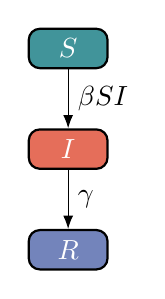
\begin{tikzpicture}[node distance=.75cm, auto,
                >=Latex, 
                every node/.append style={align=center},
                int/.style={draw, thick, minimum width=1cm,minimum height=.5cm,rounded corners}]
            
               \node [int, fill=s-color, text=white] (S)             {$S$};
               \node [int, below=of S, fill=i-color, text=white] (I) {$I$};
               \node [int, below=of I, fill=r-color, text=white] (R) {$R$};
               \coordinate[below=of I] (out);
               \path[->] (S) edge node {$\beta S I$} (I)
                         (I) edge node {$\gamma$} (out);
        \end{tikzpicture}%
        \vspace{.1cm}
         % \caption{}
         \label{fig:sir-diagram}
     \end{subfigure}%
     \hfill
     \begin{subfigure}[b]{0.3\textwidth}
         \centering
         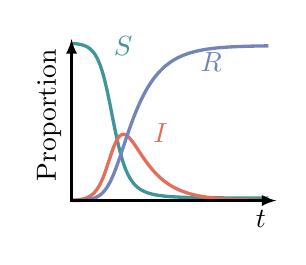
\begin{tikzpicture}[x=0.02cm,y=2cm]
      \def\xmax{130.0} % x axis maximum
      \def\ymax{1.025} % y axis maximum
      
      % CURVES
      \draw[very thick,s-color] plot[smooth] coordinates {
        (0.0, 0.998)
        (1.0, 0.9973276981931711)
        (2.0, 0.9964840728072826)
        (3.0, 0.9954259410355902)
        (4.0, 0.9940995088472758)
        (5.0, 0.9924379202498846)
        (6.0, 0.9903583301294537)
        (7.0, 0.9877584623411796)
        (8.0, 0.9845126449693982)
        (9.0, 0.9804673761499587)
        (10.0, 0.9754365737308862)
        (11.0, 0.9691968214949727)
        (12.0, 0.9614831599950985)
        (13.0, 0.9519862997172801)
        (14.0, 0.940352554204059)
        (15.0, 0.9261882782122965)
        (16.0, 0.9090710438495231)
        (17.0, 0.8885700212989189)
        (18.0, 0.8642777263133894)
        (19.0, 0.8358540642118198)
        (20.0, 0.8030810771908262)
        (21.0, 0.7659229280505638)
        (22.0, 0.7245810914666934)
        (23.0, 0.6795310390592031)
        (24.0, 0.6315262208094109)
        (25.0, 0.5815597728549975)
        (26.0, 0.530784287703032)
        (27.0, 0.480401961203948)
        (28.0, 0.4315470131997255)
        (29.0, 0.3851844173656373)
        (30.0, 0.34204311236478063)
        (31.0, 0.30259079319787735)
        (32.0, 0.26704619116159567)
        (33.0, 0.23541747963832935)
        (34.0, 0.20755337693627968)
        (35.0, 0.18319550431436243)
        (36.0, 0.16202449489961224)
        (37.0, 0.14369631108544192)
        (38.0, 0.12786819190459633)
        (39.0, 0.1142154240467327)
        (40.0, 0.10244085770765672)
        (41.0, 0.09227917117513319)
        (42.0, 0.08349762407542727)
        (43.0, 0.07589465262860504)
        (44.0, 0.06929728200938529)
        (45.0, 0.06355801522279642)
        (46.0, 0.058551620655525126)
        (47.0, 0.054172042625136994)
        (48.0, 0.050329592261200325)
        (49.0, 0.04694844269012026)
        (50.0, 0.043964461012344906)
        (51.0, 0.04132334644651637)
        (52.0, 0.038979052841522095)
        (53.0, 0.03689245949626464)
        (54.0, 0.03503025674479982)
        (55.0, 0.0333640148992419)
        (56.0, 0.03186940716069393)
        (57.0, 0.03052556194112793)
        (58.0, 0.029314522922940435)
        (59.0, 0.028220798717186017)
        (60.0, 0.027230986866564763)
        (61.0, 0.02633345947719667)
        (62.0, 0.025518099944165016)
        (63.0, 0.024776082010869227)
        (64.0, 0.024099684200702437)
        (65.0, 0.023482133047441546)
        (66.0, 0.022917471110447615)
        (67.0, 0.02240044496406817)
        (68.0, 0.021926410315262507)
        (69.0, 0.021491251208289104)
        (70.0, 0.02109131113702911)
        (71.0, 0.02072333416281497)
        (72.0, 0.0203844144502876)
        (73.0, 0.020071952916559888)
        (74.0, 0.019783619900088856)
        (75.0, 0.01951732294773462)
        (76.0, 0.019271178924476662)
        (77.0, 0.01904348983513639)
        (78.0, 0.01883272179724266)
        (79.0, 0.018637486725199447)
        (80.0, 0.018456526325907375)
        (81.0, 0.01828869811954071)
        (82.0, 0.01813296312543959)
        (83.0, 0.0179883750995347)
        (84.0, 0.017854070995352137)
        (85.0, 0.017729262582964676)
        (86.0, 0.017613229006327027)
        (87.0, 0.017505310212865357)
        (88.0, 0.017404901096874745)
        (89.0, 0.0173114462974976)
        (90.0, 0.017224435562151353)
        (91.0, 0.017143399595539257)
        (92.0, 0.01706790635057259)
        (93.0, 0.016997557715887304)
        (94.0, 0.016931986521943748)
        (95.0, 0.016870853839826203)
        (96.0, 0.016813846588184817)
        (97.0, 0.016760675318771994)
        (98.0, 0.016711072272525326)
        (99.0, 0.016664789559655245)
        (100.0, 0.016621597566351946)
        (101.0, 0.01658128346014513)
        (102.0, 0.01654364986963487)
        (103.0, 0.016508513649971912)
        (104.0, 0.01647570478322638)
        (105.0, 0.016445065355601956)
        (106.0, 0.016416448635980945)
        (107.0, 0.01638971822340957)
        (108.0, 0.01636474727181619)
        (109.0, 0.016341417776474017)
        (110.0, 0.01631961991911177)
        (111.0, 0.016299251466096593)
        (112.0, 0.01628021721595586)
        (113.0, 0.016262428496385112)
        (114.0, 0.01624580267822401)
        (115.0, 0.016230262760800425)
        (116.0, 0.016215736962871975)
        (117.0, 0.01620215835153872)
        (118.0, 0.016189464506740366)
        (119.0, 0.016177597205375163)
        (120.0, 0.016166502123166716)
        (121.0, 0.01615612857185693)
        (122.0, 0.01614642924562425)
        (123.0, 0.016137359984575585)
        (124.0, 0.016128879567973667)
        (125.0, 0.01612094950436089)
      } node[above right] at (20.0, 0.85) {$S$};
    
      \draw[very thick,i-color] plot[smooth] coordinates {
        (0.0, 0.002)
        (1.0, 0.0025118551142537743)
        (2.0, 0.0031539938777885444)
        (3.0, 0.0039591662695688465)
        (4.0, 0.004968118489808619)
        (5.0, 0.00623140960500875)
        (6.0, 0.007811562939418319)
        (7.0, 0.009785566255793595)
        (8.0, 0.012247703979930483)
        (9.0, 0.015312646690744908)
        (10.0, 0.019118631546431588)
        (11.0, 0.023830424406796634)
        (12.0, 0.029641548066158235)
        (13.0, 0.036774978103104934)
        (14.0, 0.04548115670733093)
        (15.0, 0.056031784071024576)
        (16.0, 0.06870752067429403)
        (17.0, 0.08377764007513508)
        (18.0, 0.10147010366212483)
        (19.0, 0.12193183146840725)
        (20.0, 0.14518140067848814)
        (21.0, 0.17105999575147074)
        (22.0, 0.19919043532171044)
        (23.0, 0.22895696958160838)
        (24.0, 0.259518106856763)
        (25.0, 0.28985938667094235)
        (26.0, 0.3188829532686558)
        (27.0, 0.3455194399114178)
        (28.0, 0.3688394565809396)
        (29.0, 0.3881415222032409)
        (30.0, 0.4030005812795563)
        (31.0, 0.4132730399035242)
        (32.0, 0.41906532352012577)
        (33.0, 0.42067946344958507)
        (34.0, 0.4185502560260349)
        (35.0, 0.41318559720843967)
        (36.0, 0.40511699252513234)
        (37.0, 0.39486293867085376)
        (38.0, 0.3829048359712472)
        (39.0, 0.3696734068745041)
        (40.0, 0.35554304142539545)
        (41.0, 0.34083158946059094)
        (42.0, 0.32580354734024025)
        (43.0, 0.31067510055440883)
        (44.0, 0.29561995717048395)
        (45.0, 0.28077527980532796)
        (46.0, 0.26624730330554247)
        (47.0, 0.25211645104600255)
        (48.0, 0.2384418197612011)
        (49.0, 0.22526506832660712)
        (50.0, 0.21261370867495347)
        (51.0, 0.20050387694464075)
        (52.0, 0.1889426384526646)
        (53.0, 0.17792989454199318)
        (54.0, 0.16745995095769076)
        (55.0, 0.1575228009041371)
        (56.0, 0.1481051718320928)
        (57.0, 0.13919137482870902)
        (58.0, 0.13076399175912412)
        (59.0, 0.12280442866621256)
        (60.0, 0.11529335930002195)
        (61.0, 0.10821107868483248)
        (62.0, 0.10153778306609723)
        (63.0, 0.09525378974173093)
        (64.0, 0.08933970751617225)
        (65.0, 0.08377656795680846)
        (66.0, 0.07854592336352069)
        (67.0, 0.07362991889742818)
        (68.0, 0.06901134319755721)
        (69.0, 0.06467366191877792)
        (70.0, 0.06060103750187934)
        (71.0, 0.056778337871093404)
        (72.0, 0.053191136511508266)
        (73.0, 0.04982570562316056)
        (74.0, 0.04666900390809084)
        (75.0, 0.04370866035237411)
        (76.0, 0.04093295490047132)
        (77.0, 0.03833079688115406)
        (78.0, 0.03589170191195289)
        (79.0, 0.033605767757493035)
        (80.0, 0.0314636496459622)
        (81.0, 0.029456535300379883)
        (82.0, 0.02757612011540257)
        (83.0, 0.025814582538337398)
        (84.0, 0.024164559970481298)
        (85.0, 0.022619125203910007)
        (86.0, 0.021171763595026684)
        (87.0, 0.01981635095076292)
        (88.0, 0.018547132265826043)
        (89.0, 0.017358701287442397)
        (90.0, 0.016245980943696357)
        (91.0, 0.015204204657283225)
        (92.0, 0.014228898518535435)
        (93.0, 0.013315864297351382)
        (94.0, 0.012461163329890494)
        (95.0, 0.011661101240363472)
        (96.0, 0.010912213393931912)
        (97.0, 0.0102112512067788)
        (98.0, 0.0095551691146386)
        (99.0, 0.008941112345388831)
        (100.0, 0.008366405291875594)
        (101.0, 0.007828540611958488)
        (102.0, 0.007325168898255837)
        (103.0, 0.00685408898038212)
        (104.0, 0.00641323876526587)
        (105.0, 0.00600068664013983)
        (106.0, 0.005614623366158602)
        (107.0, 0.00525335446207554)
        (108.0, 0.004915293041732614)
        (109.0, 0.004598953085528574)
        (110.0, 0.004302943118755094)
        (111.0, 0.004025960273615112)
        (112.0, 0.003766784714830889)
        (113.0, 0.003524274404150664)
        (114.0, 0.003297360197385097)
        (115.0, 0.00308504122679214)
        (116.0, 0.0028863805892277226)
        (117.0, 0.0027005012887202306)
        (118.0, 0.002526582425212876)
        (119.0, 0.0023638556598361343)
        (120.0, 0.002211601837857245)
        (121.0, 0.0020691478868978476)
        (122.0, 0.0019358638729487004)
        (123.0, 0.001811160237143461)
        (124.0, 0.0016944852515148568)
        (125.0, 0.0015853225676223741)
        } node[above right] at (45.0, 0.3) {$I$};
    
        \draw[very thick,r-color] plot[smooth] coordinates {
        (0.0, 0.0)
        (1.0, 0.00016044669257483907)
        (2.0, 0.00036193331492854905)
        (3.0, 0.0006148926948404921)
        (4.0, 0.0009323726629151103)
        (5.0, 0.001330670145106066)
        (6.0, 0.001830106931127467)
        (7.0, 0.002455971403026405)
        (8.0, 0.0032396510506710074)
        (9.0, 0.004219977159296082)
        (10.0, 0.005444794722681841)
        (11.0, 0.006972754098230427)
        (12.0, 0.00887529193874307)
        (13.0, 0.011238722179614701)
        (14.0, 0.014166289088609818)
        (15.0, 0.017779937716678768)
        (16.0, 0.022221435476182713)
        (17.0, 0.027652338625945735)
        (18.0, 0.034252170024485565)
        (19.0, 0.0422141043197727)
        (20.0, 0.05173752213068529)
        (21.0, 0.06301707619796504)
        (22.0, 0.07622847321159593)
        (23.0, 0.09151199135918818)
        (24.0, 0.10895567233382564)
        (25.0, 0.12858084047405985)
        (26.0, 0.1503327590283119)
        (27.0, 0.17407859888463387)
        (28.0, 0.1996135302193346)
        (29.0, 0.22667406043112157)
        (30.0, 0.2549563063556628)
        (31.0, 0.2841361668985982)
        (32.0, 0.31388848531827834)
        (33.0, 0.34390305691208545)
        (34.0, 0.3738963670376853)
        (35.0, 0.40361889847719784)
        (36.0, 0.4328585125752554)
        (37.0, 0.46144075024370435)
        (38.0, 0.48922697212415656)
        (39.0, 0.5161111690787633)
        (40.0, 0.542016100866948)
        (41.0, 0.566889239364276)
        (42.0, 0.5906988285843326)
        (43.0, 0.6134302468169863)
        (44.0, 0.635082760820131)
        (45.0, 0.6556667049718758)
        (46.0, 0.6752010760389326)
        (47.0, 0.6937115063288607)
        (48.0, 0.7112285879775989)
        (49.0, 0.7277864889832728)
        (50.0, 0.7434218303127018)
        (51.0, 0.7581727766088432)
        (52.0, 0.7720783087058135)
        (53.0, 0.7851776459617423)
        (54.0, 0.7975097922975096)
        (55.0, 0.8091131841966213)
        (56.0, 0.8200254210072134)
        (57.0, 0.8302830632301633)
        (58.0, 0.8399214853179355)
        (59.0, 0.8489747726166015)
        (60.0, 0.8574756538334134)
        (61.0, 0.865455461837971)
        (62.0, 0.8729441169897378)
        (63.0, 0.8799701282473998)
        (64.0, 0.8865606082831254)
        (65.0, 0.89274129899575)
        (66.0, 0.8985366055260318)
        (67.0, 0.9039696361385037)
        (68.0, 0.9090622464871803)
        (69.0, 0.913835086872933)
        (70.0, 0.9183076513610916)
        (71.0, 0.9224983279660917)
        (72.0, 0.9264244490382042)
        (73.0, 0.9301023414602796)
        (74.0, 0.9335473761918203)
        (75.0, 0.9367740166998912)
        (76.0, 0.939795866175052)
        (77.0, 0.9426257132837095)
        (78.0, 0.9452755762908044)
        (79.0, 0.9477567455173074)
        (80.0, 0.9500798240281304)
        (81.0, 0.9522547665800793)
        (82.0, 0.9542909167591578)
        (83.0, 0.9561970423621279)
        (84.0, 0.9579813690341665)
        (85.0, 0.9596516122131252)
        (86.0, 0.9612150073986462)
        (87.0, 0.9626783388363717)
        (88.0, 0.9640479666372991)
        (89.0, 0.9653298524150598)
        (90.0, 0.9665295834941521)
        (91.0, 0.9676523957471773)
        (92.0, 0.9687031951308919)
        (93.0, 0.9696865779867614)
        (94.0, 0.9706068501481657)
        (95.0, 0.9714680449198103)
        (96.0, 0.9722739400178834)
        (97.0, 0.9730280734744492)
        (98.0, 0.9737337586128361)
        (99.0, 0.9743940980949559)
        (100.0, 0.9750119971417724)
        (101.0, 0.9755901759278963)
        (102.0, 0.9761311812321092)
        (103.0, 0.9766373973696458)
        (104.0, 0.9771110564515075)
        (105.0, 0.977554248004258)
        (106.0, 0.9779689279978604)
        (107.0, 0.9783569273145148)
        (108.0, 0.9787199596864512)
        (109.0, 0.9790596291379974)
        (110.0, 0.9793774369621331)
        (111.0, 0.9796747882602882)
        (112.0, 0.9799529980692132)
        (113.0, 0.9802132970994641)
        (114.0, 0.9804568371243909)
        (115.0, 0.9806846960124074)
        (116.0, 0.9808978824479002)
        (117.0, 0.9810973403597408)
        (118.0, 0.9812839530680466)
        (119.0, 0.9814585471347885)
        (120.0, 0.981621896038976)
        (121.0, 0.9817747235412451)
        (122.0, 0.9819177068814269)
        (123.0, 0.9820514797782809)
        (124.0, 0.9821766351805113)
        (125.0, 0.9822937279280166)
        } node[above right] at (75.0, 0.75) {$R$};

        % AXES
      \draw[<->,thick]
        (\xmax,0) node[below left] {$t$}
        -| (0,\ymax) node[above left,rotate=90] {Proportion};
    \end{tikzpicture}%
    \vspace{.05cm}
         % \caption{}
         \label{fig:sir-curve}
     \end{subfigure}%
        % \bcaption{Compartmental SIR model.}{\textbf{(i)} System of differential equations representing changes in flows between compartments. \textbf{(ii)} Compartmental diagram representing flows between compartments. \textbf{(iii)} SIR dynamics over time for $\beta=0.3$ and $1/\gamma=14$.}
        % \label{fig:sir-fig}
\end{figure}

% where $\beta$ is the rate of disease transmission and $\gamma$ is the recovery rate.

% \vspace{.2cm}
% Mathematical compartmental models assume \textbf{well-mixed homogeneous populations}, meaning individual-level behaviours cannot be represented.

% \vspace{.2cm}
% Because of this, few research efforts have focused on heterogeneous protective behaviours among individuals, despite these being important for understanding how to design effective community-wide vector control interventions.

% \end{frame}
%---------------------------------------------------------

%---------------------------------------------------------
\begin{frame}
\frametitle{Agent-based modelling}

\textit{Agent-based models} (ABMs) define a population of decentralised, autonomous \textit{agents} that interact with one another to reproduce or ``grow'' emergent phenomena.

\vspace{.25cm}
An agent-based version of the \textit{SIR} (Susceptible, Infected, Recovered) model:\vspace{-.2cm}

% \addtocounter{figure}{-1}

% \begin{columns}[t]
%     \begin{column}{5cm}
%         \begin{figure}
%             \centering
%             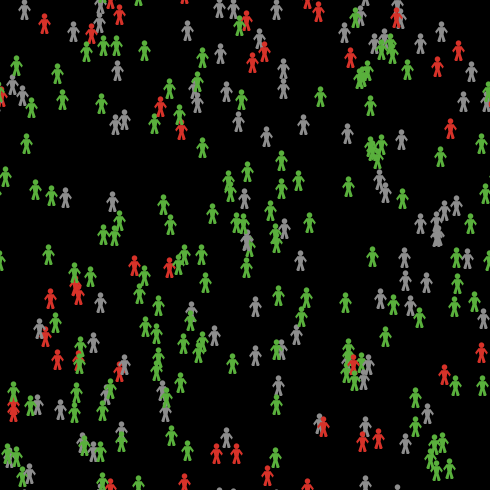
\includegraphics[width=3cm]{img/sir_agents.png}
%             \bcaption{Agent-based SIR model.}{Source: NetLogo Models Library\footnotemark[1] \cite{wilensky_netlogo_1999}.}
%         \end{figure}
%     \end{column}

%     \begin{column}{5cm}
%         \begin{figure}
    \centering
    \vspace{.4cm}
    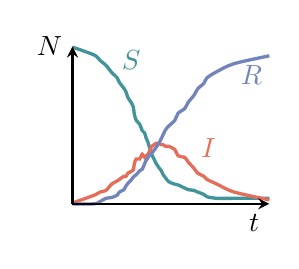
\begin{tikzpicture}[>=stealth]
    % LHS plot 1
    \draw[s-color, very thick] plot[smooth] coordinates {
    (-8.0, 3.49)
    (-7.724024512482009, 3.3899999999999997)
    (-7.6484637396372115, 3.3200000000000003)
    (-7.575293451467849, 3.26)
    (-7.503363558513278, 3.17)
    (-7.431975571153575, 3.1)
    (-7.4034740477674585, 3.04)
    (-7.347587243310602, 2.9699999999999998)
    (-7.319165044453064, 2.92)
    (-7.295761688316618, 2.85)
    (-7.256915998988681, 2.79)
    (-7.227168918566119, 2.73)
    (-7.214826797701855, 2.6399999999999997)
    (-7.190112056349427, 2.56)
    (-7.145799388697578, 2.51)
    (-7.114025393756335, 2.43)
    (-7.083940841055886, 2.4)
    (-7.065913148865518, 2.34)
    (-7.040632834972005, 2.2800000000000002)
    (-7.020523178328933, 2.21)
    (-6.994840986408573, 2.13)
    (-6.964917234604183, 2.07)
    (-6.935920958726876, 2.01)
    (-6.90240456136456, 1.96)
    (-6.871291715913282, 1.92)
    (-6.8479224101567615, 1.87)
    (-6.818213573307265, 1.83)
    (-6.776110138898, 1.78)
    (-6.700132590103333, 1.75)
    (-6.658815900705981, 1.74)
    (-6.57460720665217, 1.7)
    (-6.529765752224526, 1.68)
    (-6.45546739165365, 1.67)
    (-6.410288267674974, 1.65)
    (-6.332084009436284, 1.62)
    (-6.292160628893704, 1.59)
    (-6.164451622325407, 1.57)
    (-5.948722216423396, 1.57)
    (-5.5, 1.57)
    } node[above left,xshift=-1.5cm,yshift=1.5cm] {$S$};
    
    \draw[i-color, very thick] plot[smooth] coordinates {
    (-8.0, 1.51)
    (-7.724024512482009, 1.61)
    (-7.6484637396372115, 1.65)
    (-7.575293451467849, 1.67)
    (-7.503363558513278, 1.75)
    (-7.431975571153575, 1.79)
    (-7.4034740477674585, 1.81)
    (-7.347587243310602, 1.85)
    (-7.319165044453064, 1.85)
    (-7.295761688316618, 1.8900000000000001)
    (-7.256915998988681, 1.91)
    (-7.227168918566119, 1.93)
    (-7.214826797701855, 2.01)
    (-7.190112056349427, 2.07)
    (-7.145799388697578, 2.07)
    (-7.114025393756335, 2.13)
    (-7.083940841055886, 2.09)
    (-7.065913148865518, 2.11)
    (-7.040632834972005, 2.13)
    (-7.020523178328933, 2.17)
    (-6.994840986408573, 2.23)
    (-6.964917234604183, 2.25)
    (-6.935920958726876, 2.27)
    (-6.90240456136456, 2.27)
    (-6.871291715913282, 2.25)
    (-6.8479224101567615, 2.25)
    (-6.818213573307265, 2.23)
    (-6.776110138898, 2.23)
    (-6.700132590103333, 2.19)
    (-6.658815900705981, 2.11)
    (-6.57460720665217, 2.09)
    (-6.529765752224526, 2.0300000000000002)
    (-6.45546739165365, 1.95)
    (-6.410288267674974, 1.8900000000000001)
    (-6.332084009436284, 1.85)
    (-6.292160628893704, 1.81)
    (-6.164451622325407, 1.75)
    (-5.948722216423396, 1.65)
    (-5.5, 1.55)
    } node[above right, xshift=-1cm, yshift=.4cm] {$I$};
    
    \draw[r-color, very thick] plot[smooth] coordinates {
    (-8.0, 1.5)
    (-7.724024512482009, 1.5)
    (-7.6484637396372115, 1.53)
    (-7.575293451467849, 1.57)
    (-7.503363558513278, 1.58)
    (-7.431975571153575, 1.61)
    (-7.4034740477674585, 1.65)
    (-7.347587243310602, 1.68)
    (-7.319165044453064, 1.73)
    (-7.295761688316618, 1.76)
    (-7.256915998988681, 1.8)
    (-7.227168918566119, 1.84)
    (-7.214826797701855, 1.85)
    (-7.190112056349427, 1.87)
    (-7.145799388697578, 1.92)
    (-7.114025393756335, 1.94)
    (-7.083940841055886, 2.01)
    (-7.065913148865518, 2.05)
    (-7.040632834972005, 2.09)
    (-7.020523178328933, 2.12)
    (-6.994840986408573, 2.14)
    (-6.964917234604183, 2.18)
    (-6.935920958726876, 2.2199999999999998)
    (-6.90240456136456, 2.27)
    (-6.871291715913282, 2.33)
    (-6.8479224101567615, 2.38)
    (-6.818213573307265, 2.44)
    (-6.776110138898, 2.49)
    (-6.700132590103333, 2.56)
    (-6.658815900705981, 2.65)
    (-6.57460720665217, 2.71)
    (-6.529765752224526, 2.79)
    (-6.45546739165365, 2.88)
    (-6.410288267674974, 2.96)
    (-6.332084009436284, 3.0300000000000002)
    (-6.292160628893704, 3.1)
    (-6.164451622325407, 3.1799999999999997)
    (-5.948722216423396, 3.2800000000000002)
    (-5.5, 3.38)
    } node[above right, xshift=-.5cm, yshift=-.5cm] {$R$};
    \draw[->,thick] (-8, 1.5) -- (-5.5, 1.5) node[below left] {$t$};
    \draw[->,thick] (-8, 1.5) -- (-8, 3.5) node[left] {$N$};

    \end{tikzpicture}

    \bcaption{Stochastic output of the agent-based SIR model.}{S, I, and R plots correspond to agent disease state counts ($N$) over time ($t$).}
    \end{figure}
%     \end{column}
% \end{columns}

\begin{figure}[htbp]
   \centering
   \begin{adjustbox}{center}
   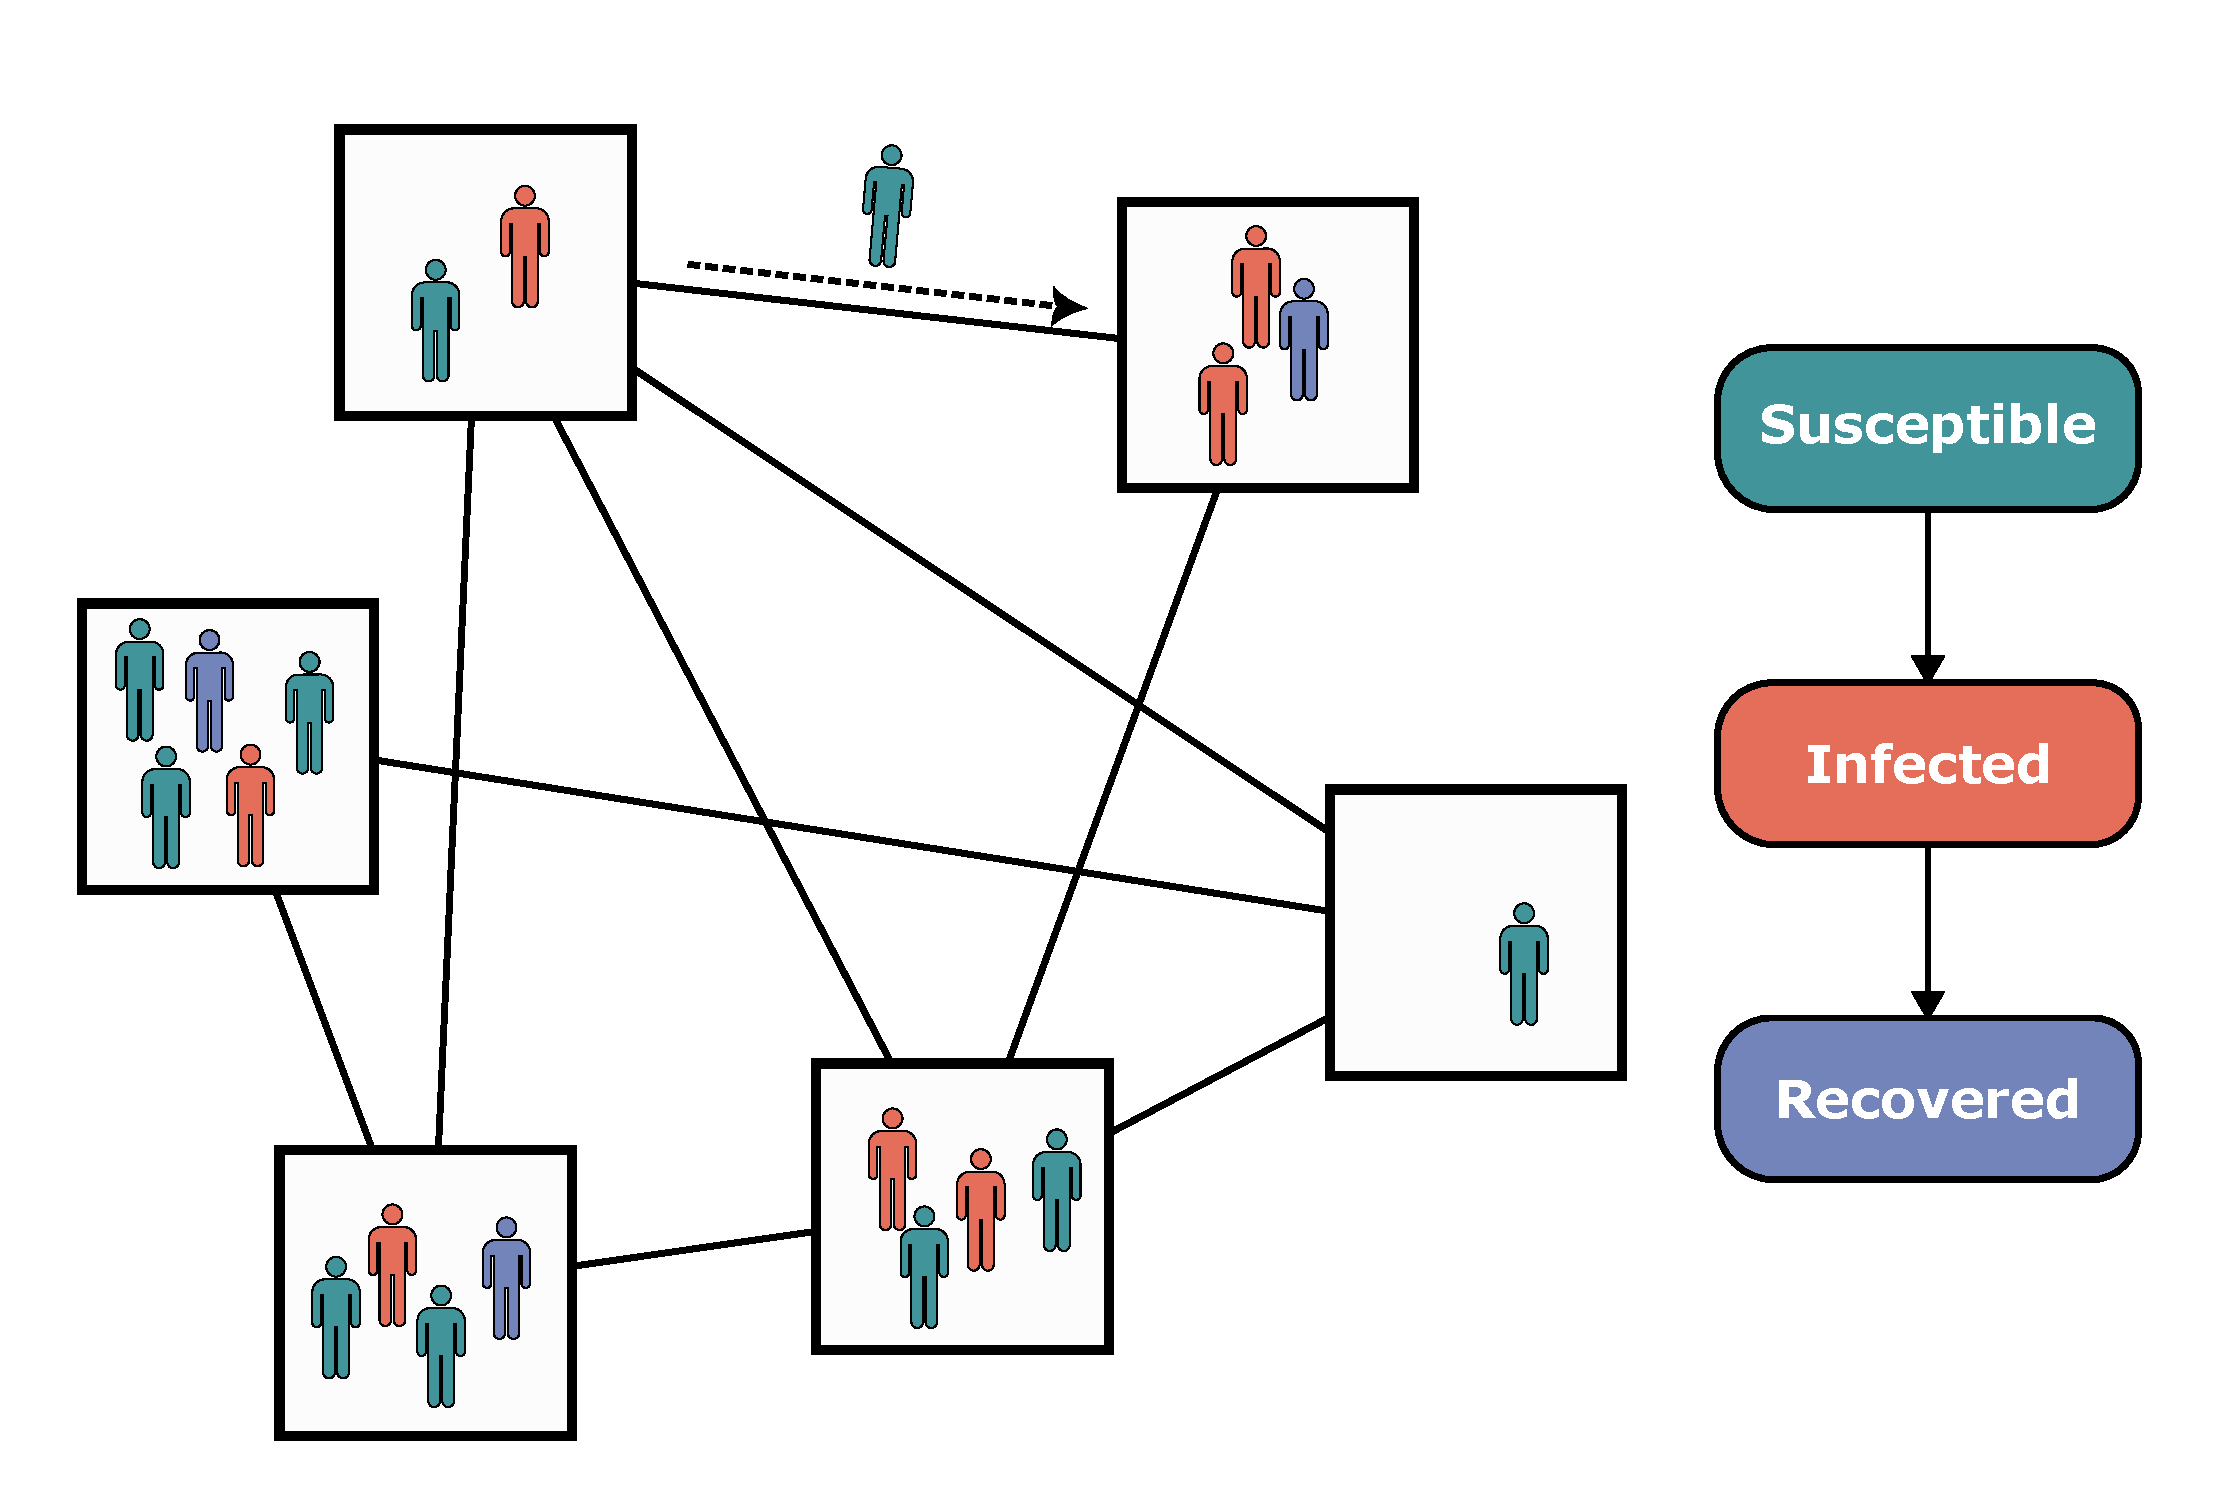
\includegraphics[width=10cm]{figs/mcs-pres-abm.pdf} 
   \end{adjustbox}
   
 % \caption{Test}
 % \label{fig:Test}
\end{figure}

% By defining system mechanisms at the \textbf{agent-level}, these models can \textbf{naturally incorporate heterogeneous factors} of individuals.

% \vspace{.2cm}
% Despite this, the implications of modelling behaviour within agent-based models is not well understood, and the impacts on disease spread are unclear.

% \footnotetext[1]{\url{https://ccl.northwestern.edu/netlogo/models/Virus}}

\end{frame}
%---------------------------------------------------------

\begin{frame}
\frametitle{Psychological behavioural theories}

% Multiple psychological behavioural theories exist for why individuals adopt preventive measures, such as the well-known Health Belief Model:

\textbf{Behavioural theories} from psychology aim to model how people behave. E.g. the Health Belief Model \cite{champion_health_2015}:

\begin{figure}
    \centering
    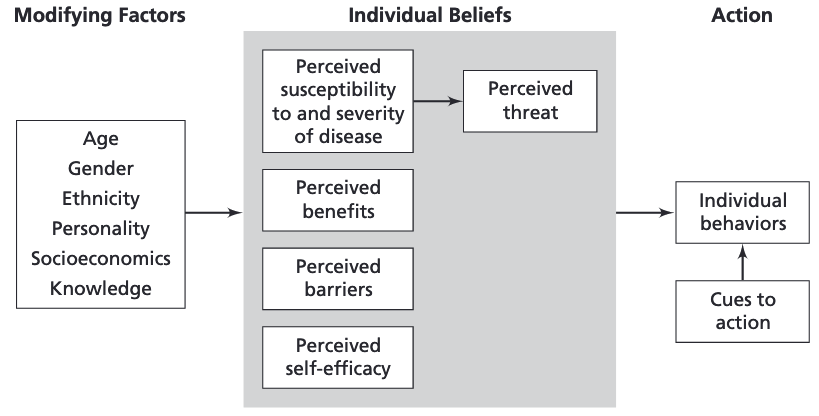
\includegraphics[width=10cm]{img/hbm.png}
    % \bcaption{Components of the Health Belief Model.}{From \textcite{champion_health_2015}.}
\end{figure}

Multiple behavioural theories exist, but few research efforts have investigated differences in system dynamics for disease spread and preventive measures when agents act according to various behavioural theories.
% This is only \textbf{one theory}, and has been criticised in the past (e.g., for ignoring social factors).

\end{frame}

%---------------------------------------------------------

% \begin{frame}
% \frametitle{Psychological behavioural theories}

% % $\dots$to examine how different behavioural theories impact disease spread and preventive behaviours, I will compare three frameworks in total.

% % \begin{columns}[h]
% %     \begin{column}{5cm}
%         \begin{figure}
%             \centering
%             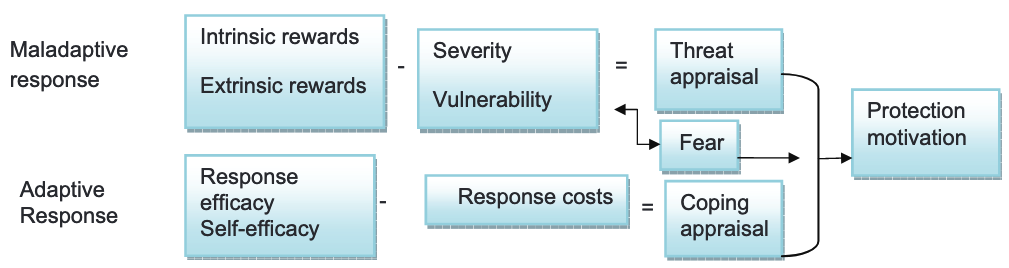
\includegraphics[width=9cm]{img/pmt.png}
%             \bcaption{Protection Motivation Theory diagram.}{From \textcite{ghahremani_effect_2014}.}
%         \end{figure}
%     % \end{column}

%     % \begin{column}{5cm}
%     \vspace{-.25cm}
%         \begin{figure}
%             \centering
%             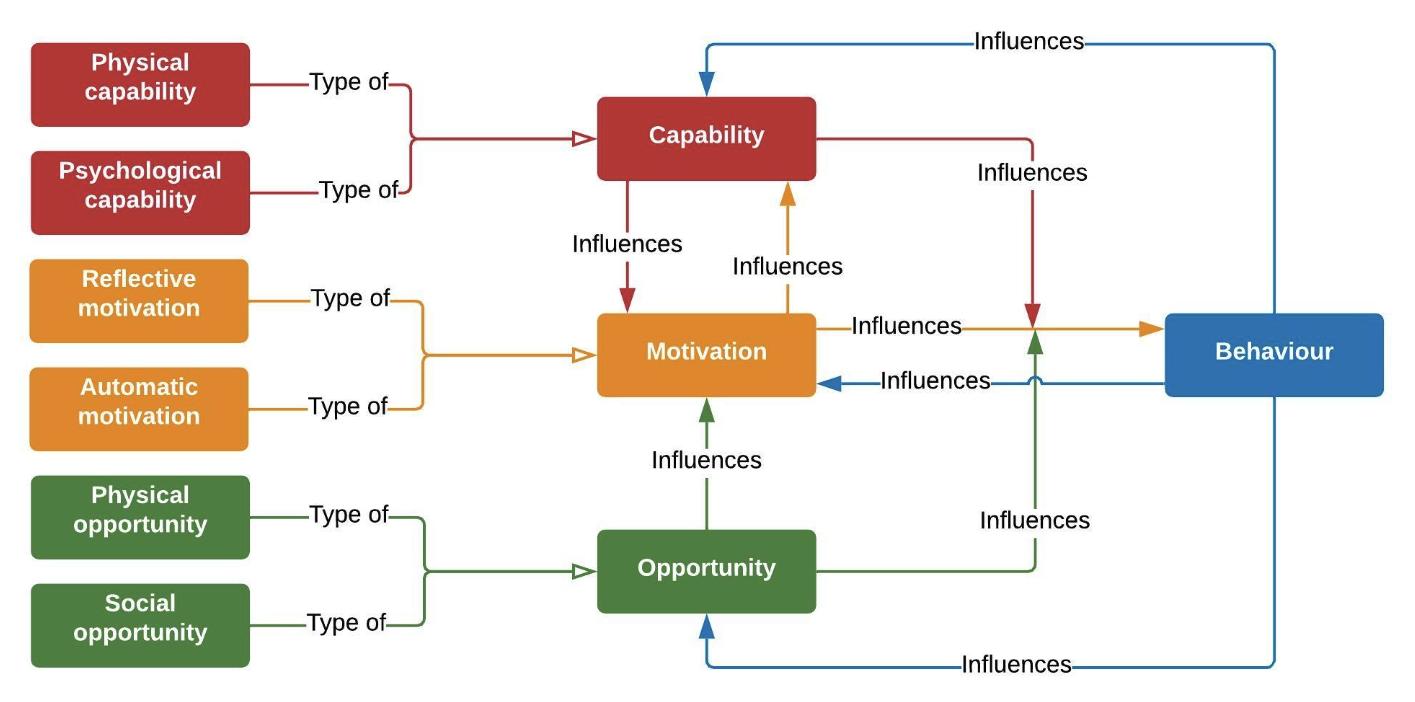
\includegraphics[width=8cm]{img/comb.png}
%             \bcaption{The COM-B (Capability, Opportunity, Motivation, and Behaviour) model.}{From \textcite{michie_behaviour_2011}.}
%         \end{figure}
% %     \end{column}
% % \end{columns}

% % This will involve computationally implementing these behavioural theories, which will be a major contribution of the project.

% % \vspace{.5cm}
% % Once I implement these, I will \alert{analytically compare their impacts on disease and preventive behaviour dynamics}.

% \end{frame}

%---------------------------------------------------------

%---------------------------------------------------------
\begin{frame}
\frametitle{Research aims and questions}

This project aims to:

\begin{enumerate}
    \item Use agent-based modelling to quantify the \textbf{effects of different behavioural theories} on the \textbf{adoption of preventive measures}.
    \item Investigate effective \textbf{strategies for community-based interventions}.
\end{enumerate}

\vspace{1cm}
Via the following research questions:

\begin{enumerate}

\item How does the choice of \alert{behavioural theory} influence the \alert{dynamics of agent-based models} for vector-borne disease spread and preventive behaviours?\label{rq1}

\item In such models, how do targeted \alert{community-based interventions} influence \alert{preventive behaviours}?\label{rq2}

\end{enumerate}


\end{frame}
%---------------------------------------------------------

\section{Approach and work completed}

\subsection{Methods}

%---------------------------------------------------------
\begin{frame}
\frametitle{Proposed methods}

% \begin{columns}
    % \begin{column}{5cm}
        \textbf{Phase 1}: Behavioural theory comparison
        \begin{enumerate}
            \item Extend an existing model \cite{manore_network-patch_2015} to incorporate preventive measures.

            \item Computationally encode three behavioural theories.
            
            \item Compare the impacts on preventive behaviours and disease spread across the three behavioural theories.
        \end{enumerate}
    % \end{column}
\vspace{1cm}
    % \begin{column}{5cm}
        \textbf{Phase 2}: Simulation of community-based interventions
        \begin{enumerate}
            \item Use the model from the first phase to simulate community-based interventions.
            \item Analyse the characteristics of effective interventions.
        \end{enumerate}
    % \end{column}
% \end{columns}

\end{frame}

%---------------------------------------------------------

%---------------------------------------------------------
\begin{frame}
\frametitle{The baseline model}

% I will extend an existing ABM that is coupled with a compartmental model for disease vectors.
Adapted from \textcite{manore_network-patch_2015}:

\begin{figure}[h]
\centering

\definecolor{cf7f7f7}{RGB}{247,247,247}
\definecolor{cc9c9c9}{RGB}{201,201,201}
\definecolor{cdfdfdf}{RGB}{223,223,223}
\definecolor{cc1c1c1}{RGB}{193,193,193}
\definecolor{c0c1024}{RGB}{12,16,36}
\definecolor{c3ea44a}{RGB}{62,164,74}
\definecolor{c2e62b0}{RGB}{46,98,176}
\definecolor{c35479c}{RGB}{53,71,156}
\definecolor{cbb7ee4}{RGB}{187,126,228}
\definecolor{c5a71fa}{RGB}{90,113,250}
\definecolor{cefef2e}{RGB}{239,239,46}
\definecolor{c14c50f}{RGB}{20,197,15}

\scalebox{0.7}{
% \adjustbox{10cm}{
\def \globalscale {1.000000}
\begin{tikzpicture}[y=1cm, x=1cm, yscale=\globalscale,xscale=\globalscale, every node/.append style={scale=\globalscale}, inner sep=0pt, outer sep=0pt]
  \path[draw=black,fill=cf7f7f7,even odd rule,line width=0.05cm] (3.3108, 14.2989) rectangle (6.5472, 8.0599);



  \path[draw=cc9c9c9,fill=white,even odd rule,line width=0.0516cm] (11.9826, 14.3339) rectangle (15.4091, 8.0581);



  \path[draw=black,fill=cdfdfdf,even odd rule,line width=0.05cm] (7.2484, 14.3349) rectangle (11.6176, 11.2963);



  \path[draw=black,fill=cc1c1c1,even odd rule,line width=0.05cm] (7.2664, 10.7569) rectangle (11.6176, 8.0599);



  \node[text=black,even odd rule,line width=0.0204cm,anchor=south west,scale=.85] (text23) at (3.355, 8.1608){$k=1$};



  \node[text=black,even odd rule,line width=0.0204cm,anchor=south west] (text23-8) at (12.1931, 13.4883){\textbf{Activities}};



  \node[text=black,even odd rule,line width=0.0204cm,anchor=south west,scale=.85] (text23-5) at (10.7, 8.1279){$k=3$};



  \node[text=black,even odd rule,line width=0.0204cm,anchor=south west,scale=.85] (text23-5-7) at (10.7, 11.3661){$k=2$};



  \node[text=black,even odd rule,line width=0.0204cm,anchor=south west] (text23-5-7-4) at (13.1675, 12.3933){Home};



  \node[text=black,even odd rule,line width=0.0204cm,anchor=south west] (text23-5-7-4-1) at (13.1611, 11.3729){Work};



  \begin{scope}[shift={(-0.7673, -2.3626)}]
    \node[text=black,even odd rule,line width=0.0204cm,anchor=south west] (text23-5-7-4-4) at (13.9321, 12.7){Shopping};



    \node[text=black,even odd rule,line width=0.0204cm,anchor=south west] (text23-5-7-4-4-8) at (13.9315, 11.7081){Recreation};



  \end{scope}
  \begin{scope}[draw=c0c1024,line cap=,line join=miter,line width=0.0369cm,cm={ 1.0333,-0.0,-0.0,-1.6099,(-0.1338, 32.7062)}]
    \path[draw=c0c1024,line cap=,line join=miter,line width=0.0369cm] (8.263, 12.4514) -- (9.7002, 12.8683);



    \path[draw=c0c1024,line cap=,line join=miter,line width=0.0369cm] (8.2433, 12.4514) -- (10.0546, 11.9459);



    \path[draw=c0c1024,line cap=,line join=miter,line width=0.0369cm] (7.8693, 14.5614) -- (5.2902, 14.6752);



    \path[draw=c0c1024,line cap=,line join=miter,line width=0.0369cm] (5.2705, 12.0597) -- (9.3852, 14.0939);



    \path[draw=c0c1024,line cap=,line join=miter,line width=0.0369cm] (7.889, 14.5614) -- (5.3296, 12.047);



    \path[draw=c0c1024,line cap=,line join=miter,line width=0.0369cm] (4.4593, 13.2515) -- (5.2875, 14.6497);



    \path[draw=c0c1024,line cap=,line join=miter,line width=0.0369cm] (5.2875, 12.0612) -- (5.3235, 14.6613);



    \path[draw=c0c1024,line cap=,line join=miter,line width=0.0369cm] (4.4773, 13.2284) -- (9.3927, 14.095);



    \path[draw=c0c1024,line cap=,line join=miter,line width=0.0369cm] (7.8443, 14.5688) -- (9.4287, 14.095);



    \path[draw=c0c1024,line cap=,line join=miter,line width=0.0369cm] (7.9163, 14.5573) -- (8.2584, 12.4541);



    \path[draw=c0c1024,line cap=,line join=miter,line width=0.0369cm] (7.8803, 14.5688) -- (10.0769, 11.9457);



    \path[draw=c0c1024,line cap=,line join=miter,line width=0.0369cm] (9.7528, 12.8586) -- (10.0229, 11.9457);



    \path[draw=c0c1024,line cap=,line join=miter,line width=0.0369cm] (5.2875, 12.0497) -- (10.0769, 11.9341);



    \path[fill=c3ea44a,nonzero rule,line cap=,line join=miter,line width=0.0004cm] (11.0475, 14.1075).. controls (11.0915, 14.2163) and (11.0435, 14.3347) .. (11.0428, 14.3365).. controls (11.0429, 14.3359) and (11.044, 14.3274) .. (11.044, 14.3274).. controls (11.0581, 14.2543) and (11.0238, 14.2131) .. (11.0238, 14.2131).. controls (11.0469, 14.2764) and (11.0042, 14.3124) .. (10.9791, 14.3274).. controls (10.9697, 14.3331) and (10.9627, 14.3379) .. (10.9627, 14.3379).. controls (10.962, 14.3379) and (10.9613, 14.3303) .. (10.9608, 14.3274).. controls (10.9439, 14.2382) and (11.0237, 14.1245) .. (11.0237, 14.1245).. controls (10.9727, 14.1536) and (10.9417, 14.2485) .. (10.9281, 14.3006).. controls (10.9443, 14.2127) and (10.9175, 14.1722) .. (10.9175, 14.1722).. controls (10.9281, 14.2457) and (10.9015, 14.3061) .. (10.8903, 14.3274).. controls (10.8875, 14.3328) and (10.8857, 14.3379) .. (10.8857, 14.3379).. controls (10.8843, 14.3379) and (10.8832, 14.3305) .. (10.8821, 14.3274).. controls (10.8629, 14.2743) and (10.8724, 14.1432) .. (10.8724, 14.1432).. controls (10.8533, 14.1738) and (10.8419, 14.2366) .. (10.8358, 14.2822).. controls (10.8358, 14.2049) and (10.798, 14.1586) .. (10.798, 14.1586).. controls (10.8379, 14.2574) and (10.7848, 14.3222) .. (10.7848, 14.3222).. controls (10.7954, 14.2336) and (10.7582, 14.2114) .. (10.7582, 14.2114).. controls (10.7857, 14.2481) and (10.7237, 14.3205) .. (10.7237, 14.3205).. controls (10.6998, 14.2251) and (10.7582, 14.0904) .. (10.7582, 14.0904).. controls (10.7228, 14.1224) and (10.7021, 14.2025) .. (10.6912, 14.2607).. controls (10.69, 14.1867) and (10.6419, 14.1586) .. (10.6419, 14.1586).. controls (10.6903, 14.2336) and (10.6414, 14.3256) .. (10.6414, 14.3256).. controls (10.6467, 14.237) and (10.6121, 14.1944) .. (10.6121, 14.1944).. controls (10.6165, 14.2335) and (10.5674, 14.3034) .. (10.5495, 14.3274).. controls (10.5456, 14.3327) and (10.5431, 14.3378) .. (10.5431, 14.3378).. controls (10.5421, 14.3378) and (10.5412, 14.3304) .. (10.5404, 14.3274).. controls (10.5226, 14.2616) and (10.559, 14.1211) .. (10.559, 14.1211).. controls (10.5172, 14.1419) and (10.4917, 14.2903) .. (10.4859, 14.3274).. controls (10.4851, 14.3328) and (10.4847, 14.3379) .. (10.4847, 14.3379).. controls (10.4844, 14.3379) and (10.4842, 14.3303) .. (10.4839, 14.3274).. controls (10.4784, 14.2698) and (10.479, 14.2059) .. (10.479, 14.2059).. controls (10.4614, 14.2183) and (10.4476, 14.3378) .. (10.4475, 14.3378) -- (10.448, 14.3274).. controls (10.4594, 14.1785) and (10.4183, 14.1296) .. (10.4183, 14.1296).. controls (10.4384, 14.2028) and (10.4021, 14.2988) .. (10.3901, 14.3274).. controls (10.3878, 14.3328) and (10.3864, 14.3378) .. (10.3864, 14.3378).. controls (10.3838, 14.3378) and (10.3815, 14.3305) .. (10.3796, 14.3274).. controls (10.3517, 14.2835) and (10.3864, 14.1824) .. (10.3864, 14.1824).. controls (10.3544, 14.2089) and (10.3434, 14.2556) .. (10.3398, 14.2905).. controls (10.3428, 14.1114) and (10.32, 14.0529) .. (10.32, 14.0529).. controls (10.3364, 14.1175) and (10.3013, 14.2878) .. (10.2927, 14.3274).. controls (10.2922, 14.3298) and (10.2922, 14.3295) .. (10.2927, 14.3274) -- (10.292, 14.3274).. controls (10.2983, 14.2671) and (10.2669, 14.1586) .. (10.2669, 14.1586).. controls (10.2669, 14.2059) and (10.25, 14.2991) .. (10.2446, 14.3274).. controls (10.2436, 14.3328) and (10.243, 14.3378) .. (10.243, 14.3378).. controls (10.2403, 14.3344) and (10.239, 14.3303) .. (10.2372, 14.3274).. controls (10.1967, 14.2503) and (10.243, 14.1211) .. (10.243, 14.1211).. controls (10.1814, 14.1739) and (10.1747, 14.2947) .. (10.1741, 14.3274).. controls (10.174, 14.3299) and (10.174, 14.3306) .. (10.1741, 14.3274).. controls (10.1741, 14.3274) and (10.1772, 14.34) .. (10.1686, 14.3274).. controls (10.139, 14.2863) and (10.1757, 14.1586) .. (10.1757, 14.1586).. controls (10.1393, 14.1834) and (10.1245, 14.2958) .. (10.1212, 14.3274).. controls (10.1207, 14.3327) and (10.12, 14.3378) .. (10.12, 14.3378).. controls (10.1191, 14.3378) and (10.1181, 14.3302) .. (10.1174, 14.3274).. controls (10.0885, 14.2187) and (10.1741, 14.0982) .. (10.1741, 14.0982).. controls (10.0892, 14.1323) and (10.0672, 14.3378) .. (10.0672, 14.3378) -- (10.0672, 14.4316) -- (11.1059, 14.4316) -- (11.1059, 14.3274) -- (11.1059, 14.3274).. controls (11.106, 14.1367) and (11.0475, 14.1075) .. (11.0475, 14.1075) -- cycle;



    \path[fill=c2e62b0,line cap=,line join=miter,line width=0.0001cm] (10.419, 14.3237).. controls (10.6757, 14.3371) and (10.846, 14.3521) .. (10.9648, 14.3716).. controls (11.0442, 14.3847) and (11.1008, 14.4015) .. (11.1248, 14.4192).. controls (11.1346, 14.4266) and (11.1419, 14.4372) .. (11.1432, 14.4459).. controls (11.1438, 14.452) and (11.1432, 14.4547) .. (11.1392, 14.4615).. controls (11.1303, 14.4774) and (11.1125, 14.4885) .. (11.0776, 14.5).. controls (11.0246, 14.5175) and (10.9605, 14.5303) .. (10.7474, 14.5658).. controls (10.5341, 14.6014) and (10.4506, 14.6208) .. (10.42, 14.6418).. controls (10.4102, 14.6485) and (10.4106, 14.6496) .. (10.4241, 14.656).. controls (10.4464, 14.6665) and (10.4907, 14.6771) .. (10.6023, 14.6985).. controls (10.7143, 14.72) and (10.7673, 14.732) .. (10.8056, 14.7442).. controls (10.8498, 14.7583) and (10.8736, 14.7713) .. (10.8866, 14.7882).. controls (10.8909, 14.7937) and (10.8914, 14.7957) .. (10.8916, 14.8059).. controls (10.8916, 14.8172) and (10.8915, 14.8175) .. (10.8839, 14.8274).. controls (10.8777, 14.8352) and (10.8731, 14.8394) .. (10.8608, 14.8474).. controls (10.8423, 14.8592) and (10.8248, 14.8669) .. (10.7937, 14.8766).. controls (10.7408, 14.8931) and (10.684, 14.9036) .. (10.5213, 14.9269).. controls (10.3269, 14.9546) and (10.2386, 14.9717) .. (10.1544, 14.9977).. controls (10.0668, 15.0247) and (10.012, 15.0531) .. (9.9641, 15.0965).. controls (9.9465, 15.1124) and (9.9185, 15.1316) .. (9.8956, 15.1434).. controls (9.8486, 15.1675) and (9.7793, 15.1902) .. (9.7024, 15.207).. controls (9.6098, 15.2271) and (9.5014, 15.2413) .. (9.3962, 15.247) -- (9.3802, 15.2479) -- (9.406, 15.2485).. controls (9.4202, 15.2488) and (9.372, 15.2493) .. (9.2988, 15.2494).. controls (9.2171, 15.2495) and (9.1628, 15.2492) .. (9.1582, 15.2485).. controls (9.1539, 15.2479) and (9.1397, 15.2466) .. (9.1265, 15.2456).. controls (9.0435, 15.2394) and (8.9661, 15.2236) .. (8.9239, 15.2043).. controls (8.8532, 15.1721) and (8.8456, 15.1277) .. (8.9016, 15.0769).. controls (8.9162, 15.0638) and (8.9592, 15.0361) .. (8.9823, 15.025).. controls (9.0774, 14.9794) and (9.2091, 14.9439) .. (9.406, 14.9109).. controls (9.4833, 14.898) and (9.5634, 14.8867) .. (9.7344, 14.8646).. controls (9.9157, 14.8413) and (9.9353, 14.8386) .. (9.9837, 14.8307).. controls (10.0446, 14.8208) and (10.0892, 14.8098) .. (10.1015, 14.8015).. controls (10.1047, 14.7995) and (10.1085, 14.7959) .. (10.1099, 14.7938).. controls (10.1122, 14.7901) and (10.1122, 14.7893) .. (10.1098, 14.786).. controls (10.1012, 14.7746) and (10.0622, 14.7642) .. (9.9622, 14.7465).. controls (9.8545, 14.7273) and (9.8162, 14.718) .. (9.7866, 14.7037).. controls (9.7585, 14.6901) and (9.7485, 14.6714) .. (9.7594, 14.6524).. controls (9.7781, 14.6201) and (9.8484, 14.5951) .. (9.9971, 14.5677).. controls (10.0848, 14.5515) and (10.166, 14.5398) .. (10.3852, 14.5114).. controls (10.5511, 14.49) and (10.5999, 14.4833) .. (10.6504, 14.4753).. controls (10.7359, 14.4619) and (10.7827, 14.4504) .. (10.7916, 14.4409).. controls (10.8026, 14.4288) and (10.7855, 14.4166) .. (10.7371, 14.4019).. controls (10.6707, 14.3817) and (10.5438, 14.362) .. (10.3887, 14.3481).. controls (10.3736, 14.3467) and (10.3585, 14.345) .. (10.3553, 14.3441).. controls (10.3433, 14.341) and (10.3414, 14.3283) .. (10.3522, 14.3237).. controls (10.3576, 14.3214) and (10.3761, 14.3214) .. (10.419, 14.3237) -- cycle;



    \begin{scope}[fill=c3ea44a,line cap=,line join=miter,line width=0.0369cm,cm={ 0.0137,-0.0,-0.0,-0.0088,(8.6487, 14.888)}]
      \begin{scope}[fill=c3ea44a,line cap=,line join=miter,line width=0.0369cm]
        \begin{scope}[fill=c3ea44a,line cap=,line join=miter,line width=0.0369cm]
          \path[fill=c3ea44a,line cap=,line join=miter,line width=0.0369cm] (71.6354, -6.7299).. controls (74.8473, -19.1172) and (71.3405, -32.6025) .. (71.2912, -32.8101).. controls (71.3, -32.7443) and (71.3785, -31.7753) .. (71.3785, -31.7753).. controls (72.4083, -23.4539) and (69.8984, -18.7605) .. (69.8984, -18.7605).. controls (71.5924, -25.9599) and (68.4665, -30.0649) .. (66.6333, -31.7753).. controls (65.9465, -32.4154) and (65.4353, -32.9619) .. (65.4353, -32.9619).. controls (65.3822, -32.9619) and (65.3354, -32.0979) .. (65.2961, -31.7753).. controls (64.0641, -21.6145) and (69.8971, -8.6719) .. (69.8971, -8.6719).. controls (66.1651, -11.9888) and (63.9045, -22.7833) .. (62.9102, -28.7226).. controls (64.0957, -18.7136) and (62.1361, -14.1039) .. (62.1361, -14.1039).. controls (62.9102, -22.4746) and (60.9658, -29.3451) .. (60.1498, -31.7753).. controls (59.9449, -32.3875) and (59.8083, -32.9619) .. (59.8083, -32.9619).. controls (59.7134, -32.9619) and (59.6287, -32.1232) .. (59.5477, -31.7753).. controls (58.146, -25.7246) and (58.838, -10.8047) .. (58.838, -10.8047).. controls (57.4465, -14.2849) and (56.6089, -21.436) .. (56.1613, -26.6266).. controls (56.1639, -17.827) and (53.4047, -12.5505) .. (53.4047, -12.5505).. controls (56.3156, -23.8043) and (52.4345, -31.1769) .. (52.4345, -31.1769).. controls (53.2098, -21.0882) and (50.4939, -18.5658) .. (50.4939, -18.5658).. controls (52.5002, -22.7416) and (47.9715, -30.9847) .. (47.9715, -30.9847).. controls (46.2258, -20.1193) and (50.4939, -4.7895) .. (50.4939, -4.7895).. controls (47.9094, -8.4315) and (46.3926, -17.5474) .. (45.5982, -24.175).. controls (45.5134, -15.7561) and (41.9978, -12.5505) .. (41.9978, -12.5505).. controls (45.5311, -21.0882) and (41.9572, -31.5653) .. (41.9572, -31.5653).. controls (42.3458, -21.4765) and (39.8219, -16.6239) .. (39.8219, -16.6239).. controls (40.1393, -21.0782) and (36.5491, -29.0441) .. (35.2437, -31.7741).. controls (34.9565, -32.3724) and (34.7768, -32.9607) .. (34.7768, -32.9607).. controls (34.7022, -32.9607) and (34.639, -32.1093) .. (34.5808, -31.7741).. controls (33.2765, -24.28) and (35.9407, -8.2811) .. (35.9407, -8.2811).. controls (32.8869, -10.6568) and (31.0197, -27.5527) .. (30.5984, -31.7754).. controls (30.5377, -32.3839) and (30.5074, -32.9621) .. (30.5074, -32.9621).. controls (30.4897, -32.9621) and (30.4694, -32.0967) .. (30.4505, -31.7754).. controls (30.0482, -25.2162) and (30.0925, -17.9384) .. (30.0925, -17.9384).. controls (28.8085, -19.3477) and (27.7965, -32.9607) .. (27.7901, -32.9607) -- (27.8242, -31.7741).. controls (28.6591, -14.8238) and (25.656, -9.2526) .. (25.656, -9.2526).. controls (27.1259, -17.5804) and (24.4718, -28.5192) .. (23.5965, -31.7741).. controls (23.432, -32.3876) and (23.3283, -32.9607) .. (23.3283, -32.9607).. controls (23.136, -32.9607) and (22.9715, -32.127) .. (22.8273, -31.7741).. controls (20.7894, -26.7773) and (23.3283, -15.2666) .. (23.3283, -15.2666).. controls (20.9854, -18.2774) and (20.1847, -23.593) .. (19.9241, -27.5716).. controls (20.1392, -7.1829) and (18.4769, -0.52) .. (18.4769, -0.52).. controls (19.6724, -7.8724) and (17.1044, -27.2629) .. (16.4769, -31.7741).. controls (16.4403, -32.0399) and (16.444, -32.0119) .. (16.4769, -31.7741) -- (16.4264, -31.7741).. controls (16.8906, -24.91) and (14.5959, -12.5505) .. (14.5959, -12.5505).. controls (14.5959, -17.9384) and (13.3587, -28.547) .. (12.9678, -31.7741).. controls (12.8943, -32.3813) and (12.8502, -32.9607) .. (12.8502, -32.9607).. controls (12.6516, -32.5648) and (12.5554, -32.1006) .. (12.4238, -31.7741).. controls (9.4673, -22.9908) and (12.8502, -8.2811) .. (12.8502, -8.2811).. controls (8.3443, -14.2899) and (7.8572, -28.0458) .. (7.8104, -31.7739).. controls (7.8065, -32.0611) and (7.8053, -32.1396) .. (7.8104, -31.7739).. controls (7.8104, -31.7739) and (8.0406, -33.201) .. (7.4094, -31.7739).. controls (5.245, -27.097) and (7.9293, -12.5504) .. (7.9293, -12.5504).. controls (5.2701, -15.3765) and (4.1886, -28.1698) .. (3.9496, -31.7739).. controls (3.9104, -32.3748) and (3.8611, -32.9606) .. (3.8611, -32.9606).. controls (3.7952, -32.9606) and (3.7232, -32.0941) .. (3.6687, -31.7739).. controls (1.5573, -19.393) and (7.8142, -5.6799) .. (7.8142, -5.6799).. controls (1.6067, -9.5611) and (0.0, -32.9593) .. (0.0, -32.9593) -- (0.0, -43.6326) -- (75.9023, -43.6326) -- (75.9023, -31.7739) -- (75.9023, -31.7739).. controls (75.9137, -10.0558) and (71.6354, -6.7299) .. (71.6354, -6.7299) -- cycle;



        \end{scope}
      \end{scope}
    \end{scope}
    \begin{scope}[fill=c3ea44a,line cap=,line join=miter,line width=0.0369cm,cm={ 0.0137,-0.0,-0.0,-0.0088,(9.3372, 14.8826)}]
      \begin{scope}[fill=c3ea44a,line cap=,line join=miter,line width=0.0369cm]
        \begin{scope}[fill=c3ea44a,line cap=,line join=miter,line width=0.0369cm]
          \path[fill=c3ea44a,line cap=,line join=miter,line width=0.0369cm] (71.6354, -6.7299).. controls (74.8473, -19.1172) and (71.3405, -32.6025) .. (71.2912, -32.8101).. controls (71.3, -32.7443) and (71.3785, -31.7753) .. (71.3785, -31.7753).. controls (72.4083, -23.4539) and (69.8984, -18.7605) .. (69.8984, -18.7605).. controls (71.5924, -25.9599) and (68.4665, -30.0649) .. (66.6333, -31.7753).. controls (65.9465, -32.4154) and (65.4353, -32.9619) .. (65.4353, -32.9619).. controls (65.3822, -32.9619) and (65.3354, -32.0979) .. (65.2961, -31.7753).. controls (64.0641, -21.6145) and (69.8971, -8.6719) .. (69.8971, -8.6719).. controls (66.1651, -11.9888) and (63.9045, -22.7833) .. (62.9102, -28.7226).. controls (64.0957, -18.7136) and (62.1361, -14.1039) .. (62.1361, -14.1039).. controls (62.9102, -22.4746) and (60.9658, -29.3451) .. (60.1498, -31.7753).. controls (59.9449, -32.3875) and (59.8083, -32.9619) .. (59.8083, -32.9619).. controls (59.7134, -32.9619) and (59.6287, -32.1232) .. (59.5477, -31.7753).. controls (58.146, -25.7246) and (58.838, -10.8047) .. (58.838, -10.8047).. controls (57.4465, -14.2849) and (56.6089, -21.436) .. (56.1613, -26.6266).. controls (56.1639, -17.827) and (53.4047, -12.5505) .. (53.4047, -12.5505).. controls (56.3156, -23.8043) and (52.4345, -31.1769) .. (52.4345, -31.1769).. controls (53.2098, -21.0882) and (50.4939, -18.5658) .. (50.4939, -18.5658).. controls (52.5002, -22.7416) and (47.9715, -30.9847) .. (47.9715, -30.9847).. controls (46.2258, -20.1193) and (50.4939, -4.7895) .. (50.4939, -4.7895).. controls (47.9094, -8.4315) and (46.3926, -17.5474) .. (45.5982, -24.175).. controls (45.5134, -15.7561) and (41.9978, -12.5505) .. (41.9978, -12.5505).. controls (45.5311, -21.0882) and (41.9572, -31.5653) .. (41.9572, -31.5653).. controls (42.3458, -21.4765) and (39.8219, -16.6239) .. (39.8219, -16.6239).. controls (40.1393, -21.0782) and (36.5491, -29.0441) .. (35.2437, -31.7741).. controls (34.9565, -32.3724) and (34.7768, -32.9607) .. (34.7768, -32.9607).. controls (34.7022, -32.9607) and (34.639, -32.1093) .. (34.5808, -31.7741).. controls (33.2765, -24.28) and (35.9407, -8.2811) .. (35.9407, -8.2811).. controls (32.8869, -10.6568) and (31.0197, -27.5527) .. (30.5984, -31.7754).. controls (30.5377, -32.3839) and (30.5074, -32.9621) .. (30.5074, -32.9621).. controls (30.4897, -32.9621) and (30.4694, -32.0967) .. (30.4505, -31.7754).. controls (30.0482, -25.2162) and (30.0925, -17.9384) .. (30.0925, -17.9384).. controls (28.8085, -19.3477) and (27.7965, -32.9607) .. (27.7901, -32.9607) -- (27.8242, -31.7741).. controls (28.6591, -14.8238) and (25.656, -9.2526) .. (25.656, -9.2526).. controls (27.1259, -17.5804) and (24.4718, -28.5192) .. (23.5965, -31.7741).. controls (23.432, -32.3876) and (23.3283, -32.9607) .. (23.3283, -32.9607).. controls (23.136, -32.9607) and (22.9715, -32.127) .. (22.8273, -31.7741).. controls (20.7894, -26.7773) and (23.3283, -15.2666) .. (23.3283, -15.2666).. controls (20.9854, -18.2774) and (20.1847, -23.593) .. (19.9241, -27.5716).. controls (20.1392, -7.1829) and (18.4769, -0.52) .. (18.4769, -0.52).. controls (19.6724, -7.8724) and (17.1044, -27.2629) .. (16.4769, -31.7741).. controls (16.4403, -32.0399) and (16.444, -32.0119) .. (16.4769, -31.7741) -- (16.4264, -31.7741).. controls (16.8906, -24.91) and (14.5959, -12.5505) .. (14.5959, -12.5505).. controls (14.5959, -17.9384) and (13.3587, -28.547) .. (12.9678, -31.7741).. controls (12.8943, -32.3813) and (12.8502, -32.9607) .. (12.8502, -32.9607).. controls (12.6516, -32.5648) and (12.5554, -32.1006) .. (12.4238, -31.7741).. controls (9.4673, -22.9908) and (12.8502, -8.2811) .. (12.8502, -8.2811).. controls (8.3443, -14.2899) and (7.8572, -28.0458) .. (7.8104, -31.7739).. controls (7.8065, -32.0611) and (7.8053, -32.1396) .. (7.8104, -31.7739).. controls (7.8104, -31.7739) and (8.0406, -33.201) .. (7.4094, -31.7739).. controls (5.245, -27.097) and (7.9293, -12.5504) .. (7.9293, -12.5504).. controls (5.2701, -15.3765) and (4.1886, -28.1698) .. (3.9496, -31.7739).. controls (3.9104, -32.3748) and (3.8611, -32.9606) .. (3.8611, -32.9606).. controls (3.7952, -32.9606) and (3.7232, -32.0941) .. (3.6687, -31.7739).. controls (1.5573, -19.393) and (7.8142, -5.6799) .. (7.8142, -5.6799).. controls (1.6067, -9.5611) and (0.0, -32.9593) .. (0.0, -32.9593) -- (0.0, -43.6326) -- (75.9023, -43.6326) -- (75.9023, -31.7739) -- (75.9023, -31.7739).. controls (75.9137, -10.0558) and (71.6354, -6.7299) .. (71.6354, -6.7299) -- cycle;



        \end{scope}
      \end{scope}
    \end{scope}
  \end{scope}
  \path[draw=c35479c,fill=cbb7ee4,even odd rule,line cap=butt,line width=0.0691cm,cm={ 0.5435,-0.0,-0.0,0.6169,(2.434, 4.3603)}] (6.0592, 7.2087) -- (5.4316, 7.2059) -- (4.8039, 7.2031) -- (5.1153, 7.7481) -- (5.4267, 8.293) -- (5.743, 7.7508) -- cycle;



  \path[draw=c35479c,fill=cbb7ee4,even odd rule,line cap=butt,line width=0.0691cm,cm={ 0.5435,-0.0,-0.0,0.6169,(9.6407, 5.75)}] (6.0592, 7.2087) -- (5.4316, 7.2059) -- (4.8039, 7.2031) -- (5.1153, 7.7481) -- (5.4267, 8.293) -- (5.743, 7.7508) -- cycle;



  \path[draw=c35479c,fill=c5a71fa,line width=0.0491cm,cm={ 0.8199,-0.0,-0.0,0.8199,(-1.4848, 2.4002)}] (7.6283, 10.5047) -- (7.3391, 10.6633) -- (7.0445, 10.515) -- (7.106, 10.839) -- (6.8739, 11.0733) -- (7.2011, 11.115) -- (7.3522, 11.4081) -- (7.4929, 11.1098) -- (7.8184, 11.0567) -- (7.5782, 10.8307) -- cycle;



  \path[draw=c35479c,fill=c5a71fa,line width=0.0491cm,cm={ 0.8199,-0.0,-0.0,0.8199,(4.2447, 4.5068)}] (7.6283, 10.5047) -- (7.3391, 10.6633) -- (7.0445, 10.515) -- (7.106, 10.839) -- (6.8739, 11.0733) -- (7.2011, 11.115) -- (7.3522, 11.4081) -- (7.4929, 11.1098) -- (7.8184, 11.0567) -- (7.5782, 10.8307) -- cycle;



  \path[draw=c35479c,fill=c5a71fa,line width=0.0491cm,cm={ 0.8199,-0.0,-0.0,0.8199,(6.5942, 3.5507)}] (7.6283, 10.5047) -- (7.3391, 10.6633) -- (7.0445, 10.515) -- (7.106, 10.839) -- (6.8739, 11.0733) -- (7.2011, 11.115) -- (7.3522, 11.4081) -- (7.4929, 11.1098) -- (7.8184, 11.0567) -- (7.5782, 10.8307) -- cycle;



  \path[draw=c35479c,fill=c5a71fa,line width=0.0491cm,cm={ 0.8199,-0.0,-0.0,0.8199,(2.3783, 3.6635)}] (7.6283, 10.5047) -- (7.3391, 10.6633) -- (7.0445, 10.515) -- (7.106, 10.839) -- (6.8739, 11.0733) -- (7.2011, 11.115) -- (7.3522, 11.4081) -- (7.4929, 11.1098) -- (7.8184, 11.0567) -- (7.5782, 10.8307) -- cycle;



  \path[draw=c35479c,fill=c5a71fa,line width=0.0491cm,cm={ 0.8199,-0.0,-0.0,0.8199,(3.5926, 1.0508)}] (7.6283, 10.5047) -- (7.3391, 10.6633) -- (7.0445, 10.515) -- (7.106, 10.839) -- (6.8739, 11.0733) -- (7.2011, 11.115) -- (7.3522, 11.4081) -- (7.4929, 11.1098) -- (7.8184, 11.0567) -- (7.5782, 10.8307) -- cycle;



  \path[draw=c35479c,fill=cefef2e,line cap=butt,line width=0.0402cm,cm={ 1.1141,-0.0,-0.0,1.1141,(1.1802, -2.175)}] (3.9667, 13.556) -- (3.5553, 13.5593) -- (3.4313, 13.9516) -- (3.7661, 14.1908) -- (4.097, 13.9463) -- cycle;



  \path[draw=c35479c,fill=cefef2e,line cap=butt,line width=0.0402cm,cm={ 1.1141,-0.0,-0.0,1.1141,(5.7913, -3.4734)}] (3.9667, 13.556) -- (3.5553, 13.5593) -- (3.4313, 13.9516) -- (3.7661, 14.1908) -- (4.097, 13.9463) -- cycle;



  \path[draw=c35479c,fill=cefef2e,line cap=butt,line width=0.0402cm,cm={ 1.1141,-0.0,-0.0,1.1141,(8.4107, -3.9224)}] (3.9667, 13.556) -- (3.5553, 13.5593) -- (3.4313, 13.9516) -- (3.7661, 14.1908) -- (4.097, 13.9463) -- cycle;



  \path[draw=c35479c,fill=c14c50f,line cap=butt,line width=0.037cm] (7.6904, 9.5706) rectangle (8.3836, 8.8961);



  \path[draw=c35479c,fill=c14c50f,line cap=butt,line width=0.037cm] (12.2452, 9.7887) rectangle (12.9384, 9.1142);

% SEI
\node[draw, thick, minimum width=1cm, minimum height=1cm] (S) at (1.3, 13.1) {$S_v$};
\node[draw, thick, minimum width=1cm, minimum height=1cm, below=1cm of S] (E) {$E_v$};
\node[draw, thick, minimum width=1cm, minimum height=1cm, below=1cm of E] (I) {$I_v$};

\coordinate[above=1cm of S] (in);
\coordinate[below=1cm of I] (out);

\coordinate[below left=1cm of S] (Sd);
\coordinate[below left=1cm of E] (Ed);
\coordinate[below left=1cm of I] (Id);

% \coordinate[right=2.1cm of S] (abm-out);

\coordinate[below=.5cm of S] (mid-se);
\coordinate[right=2.6cm of mid-se] (abm-out);
\coordinate[right=2.1cm of I] (abm-in);

\coordinate[right=3.425cm of I] (triangle-in);
\coordinate[right=2.5cm of I,yshift=2.1cm] (star-in);

\node[left=.6cm of in,yshift=.3cm] (a) {\textbf{(a)}};
\node[right=2.6cm of a] {\textbf{(b)}};

\path[->, very thick]   (in) edge node [right, xshift=.1cm] {$h_v(N_v,t)$} (S)
                        (S) edge node {} (E)
                        (E) edge node [right, xshift=.1cm] {$\nu_v$} (I)
                        (S) edge node [above left] {$\mu_v$} (Sd)
                        (E) edge node [above left] {$\mu_v$} (Ed)
                        (I) edge node [above left] {$\mu_v$} (Id);

\path[->, very thick, dashed] (I) edge node [above, yshift=.1cm, xshift=.5cm] {$\lambda_{h,j}$} (triangle-in)
                              (I) edge node [above, yshift=.05cm, xshift=-.3cm] {$\lambda_{h,j}$} (star-in)
                              (abm-out) edge node [above, yshift=.1cm] {$\lambda_v$} (mid-se);

% \begin{tikzpicture}[node distance=1cm, auto,
%                 >=Latex, 
%                 every node/.append style={align=center},
%                 int/.style={draw, thick, minimum width=2cm,minimum height=.6cm,rounded corners}]
            
%                \node [int, fill=s-color, text=white] (S)             {$S$};
%                \node [int, below=of S, fill=i-color, text=white] (I) {$I$};
%                \node [int, below=of I, fill=r-color, text=white] (R) {$R$};
%                \coordinate[below=of I] (out);
%                \path[->] (S) edge node {$\beta S I$} (I)
%                          (I) edge node {$\gamma$} (out);
%         \end{tikzpicture}



\end{tikzpicture}
}
% }

% \bcaption{Network-patch architecture for the model.}{}
\label{fig:manore-abm}
\end{figure}
%
\vspace{-.4cm}
\begin{itemize}
    \item \textbf{(a)} Mosquito model.
    \item \textbf{(b)} Agent-based model.
\end{itemize}
 % $\lambda_v,\lambda_{h,j}$ couple the two models: infectious agents from the network ABM shown in \textbf{(b)} supply infection force on vectors ($\lambda_v$), and the compartmental model communicates the infection force on agents $\lambda_{h,j}$ in activity $j$.

\end{frame}

%---------------------------------------------------------

%---------------------------------------------------------
% \begin{frame}
% \frametitle{Phase 2: Targeted community-based interventions}

% Simulations of community-based interventions will directly and indirectly affect behavioural theory compartments:

% \begin{figure}[h]
%    \centering
%    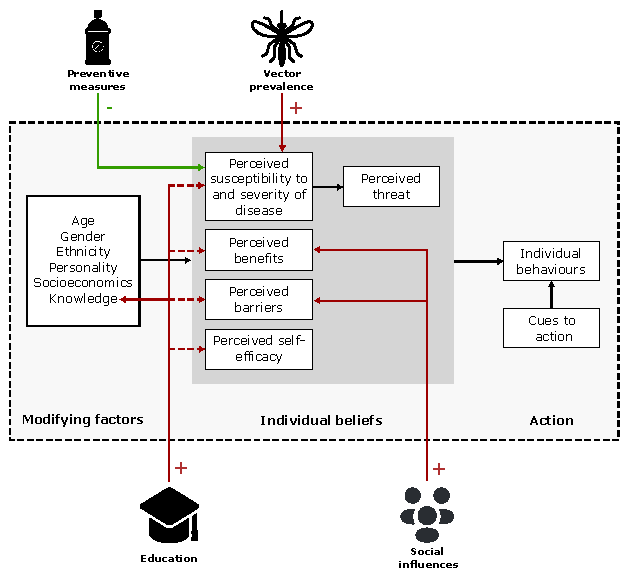
\includegraphics[width=8cm]{figs/hbm-cbi.pdf}
%  % \caption{Test}
%  % \label{fig:Test}
% \end{figure}

% \end{frame}

%---------------------------------------------------------

\subsection{Work completed}

%---------------------------------------------------------
\begin{frame}
\frametitle{Reproducing the baseline model}

\begin{columns}[h]

    \begin{column}{10cm}
        \begin{figure}[h]
           \centering
           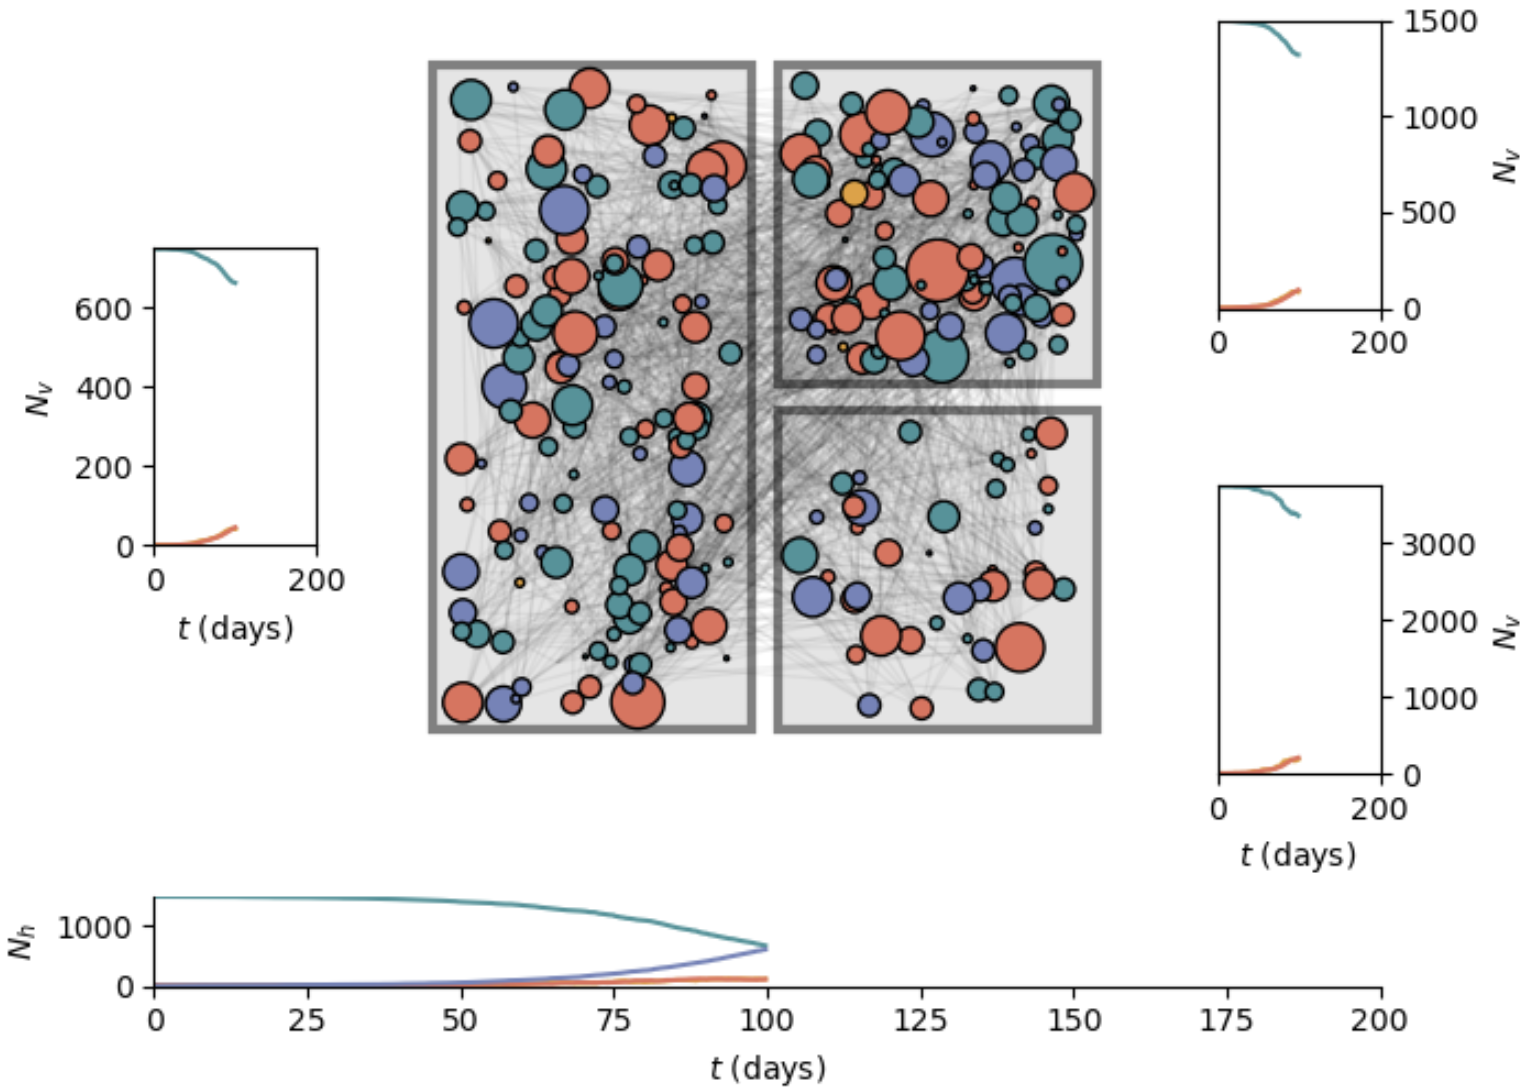
\includegraphics[width=10cm]{figs/vis.png}
         % \bcaption{Visualisation for baseline reproduced model.}{}
         % \label{fig:Test}
        \end{figure}
    \end{column}
    
    \begin{column}{2cm}
        \begin{figure}
            \centering
            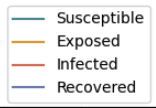
\includegraphics[width=2cm]{figs/vis_labels.png}
        \end{figure}
    \end{column}

\end{columns}


\end{frame}

%---------------------------------------------------------

%---------------------------------------------------------
\begin{frame}
\frametitle{Reproducing the baseline model}


% \begin{figure}[h]
%    \centering
%    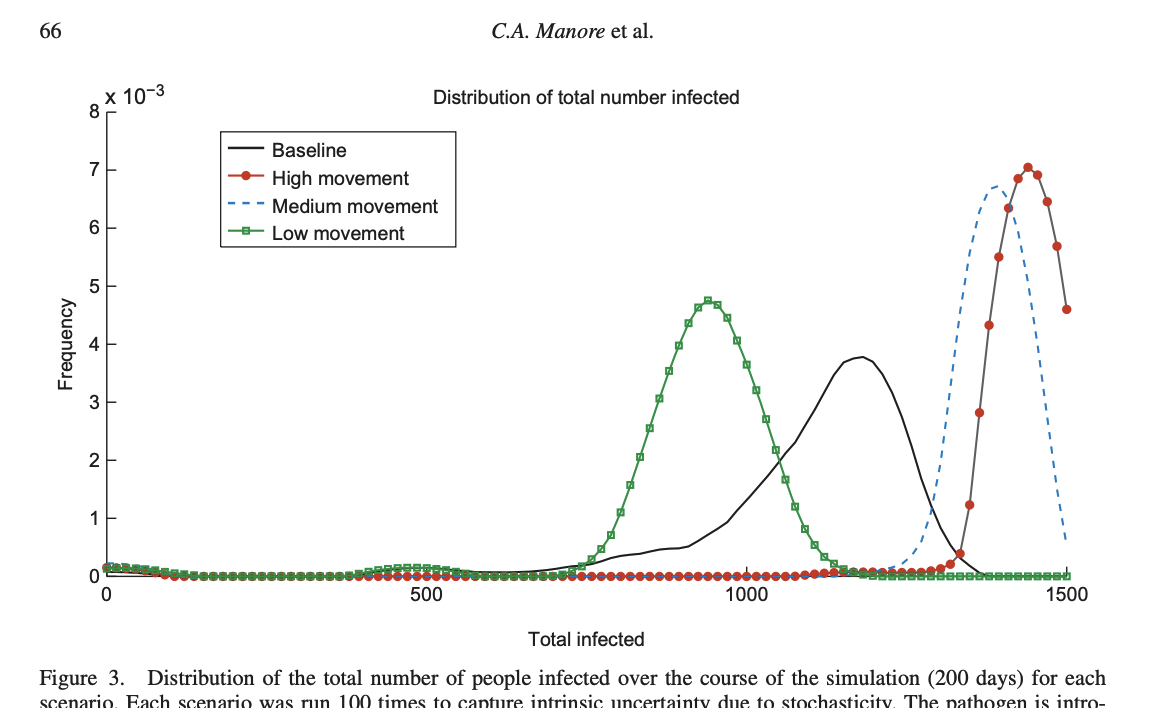
\includegraphics[width=7cm]{figs/repr_original.png}
%  \caption*{Figure from original paper \cite{manore_network-patch_2015}.}
%  % \label{fig:Test}
% \end{figure}

% \begin{figure}[h]
%    \centering
%    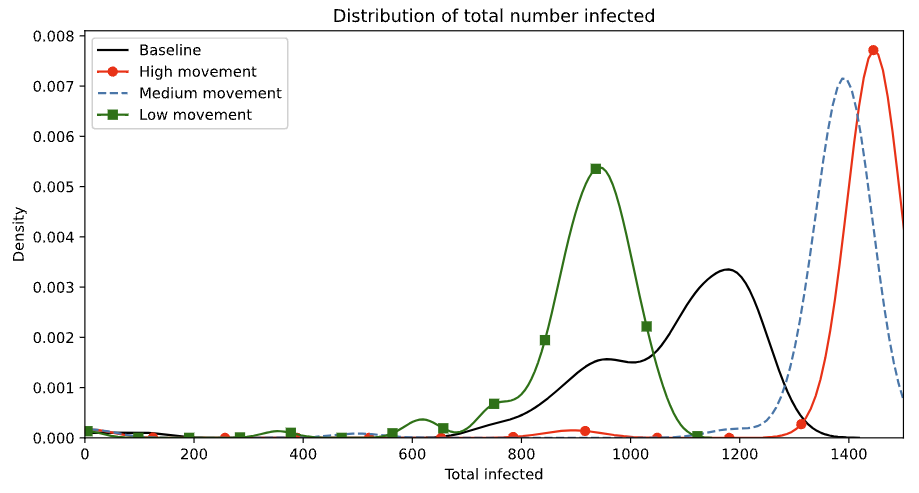
\includegraphics[width=7cm]{figs/repr_repr.png}
%  \caption*{Reproduced figure from simulations.}
%  % \label{fig:Test}
% \end{figure}

\begin{columns}[h]

    \begin{column}{6cm}
        \begin{figure}[h]
   \centering
   \fbox{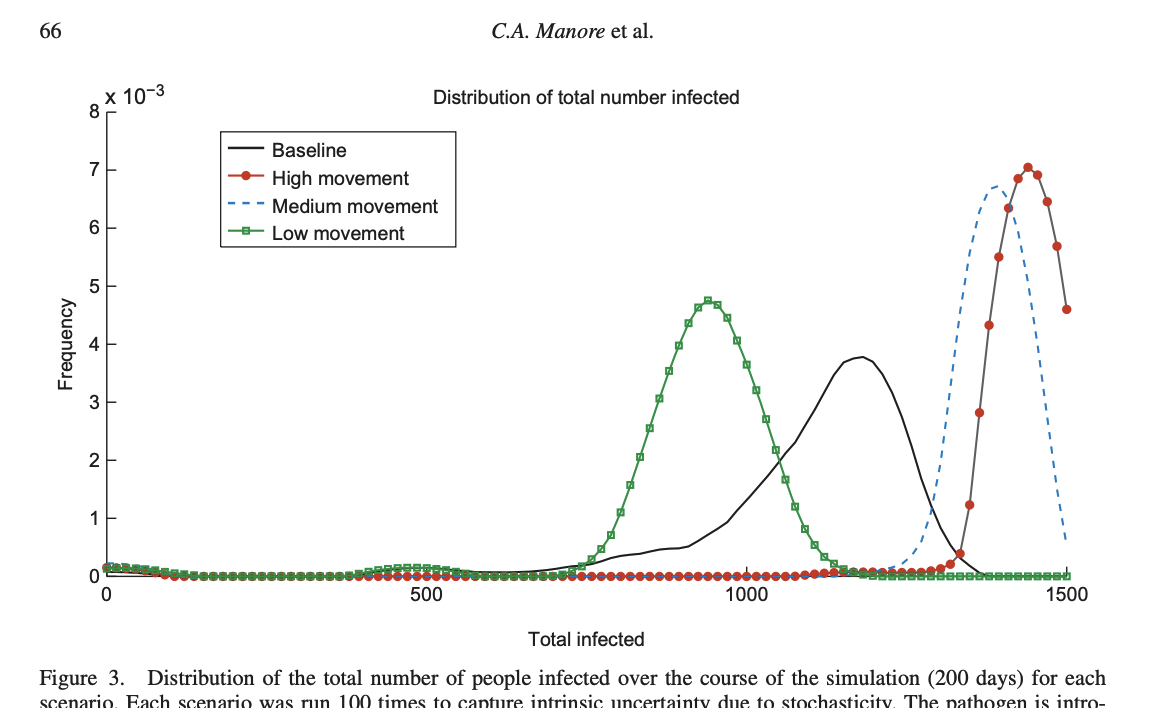
\includegraphics[width=6cm]{figs/repr_original.png}}
 \caption*{Figure from original paper \cite{manore_network-patch_2015}.}
 % \label{fig:Test}
\end{figure}
    \end{column}

    


    
    \begin{column}{6cm}
        \begin{figure}[h]
   \centering
   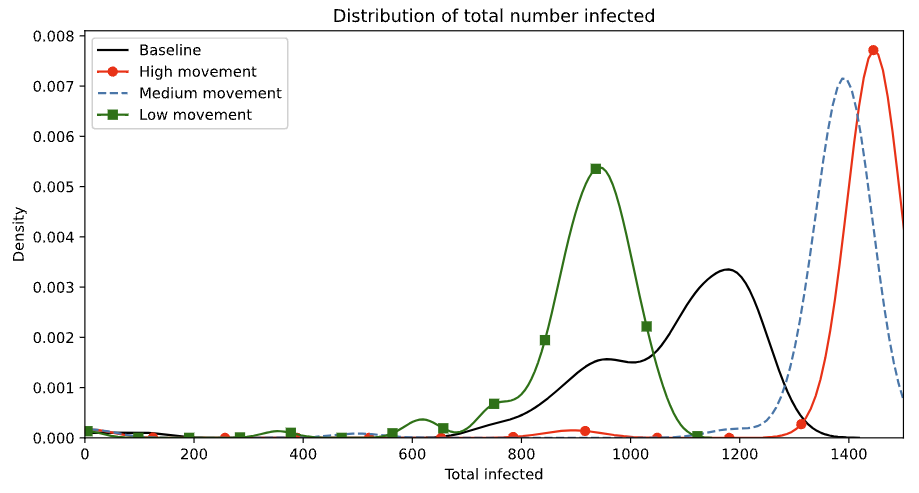
\includegraphics[width=6cm]{figs/repr_repr.png}
 \caption*{Reproduced figure from simulations.}
 % \label{fig:Test}
\end{figure}
    \end{column}

\end{columns}


\end{frame}

%---------------------------------------------------------

\section{Future work}

\subsection{Contributions}

%---------------------------------------------------------
\begin{frame}
\frametitle{Research timeline}

To achieve the research objectives within the required timeframe, I propose the following timeline:

\begin{figure}[htbp]
   \centering
   \begin{adjustbox}{center}
   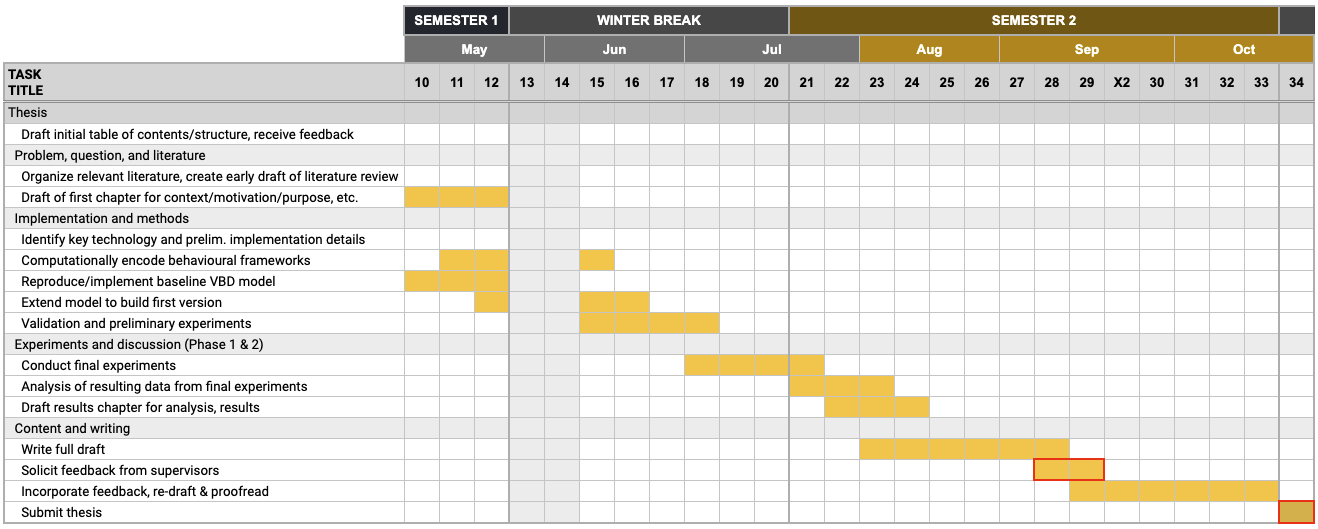
\includegraphics[width=12cm]{figs/mcs-pres-research-timeline.png} 
   \end{adjustbox}
   
 % \caption{Test}
 % \label{fig:Test}
\end{figure}

\end{frame}

%---------------------------------------------------------

%---------------------------------------------------------
\begin{frame}
\frametitle{Expected contributions and implications}

This project will contribute a \alert{methodological contribution} to the modelling community and an \alert{investigation into an understudied area of research} in the field of vector-borne diseases:

\vspace{.5cm}
\textbf{Phase 1} will contribute:

\begin{enumerate}
    \item an extension of an existing agent-based model with computational implementations of three psychological behavioural theories;
    % \item computational implementations of three behavioural theories (including the novel \textit{COM-B}); and
    \item insights into how these decision-making processes affect the dynamics between disease spread and preventive behaviours.
\end{enumerate}

\vspace{.5cm}
\textbf{Phase 2} will contribute:

\begin{enumerate}
    \item an analysis of intervention characteristics that effectively promote preventive behaviours and curb disease spread.
\end{enumerate}

\end{frame}

\subsection{Questions}

%---------------------------------------------------------
\begin{frame}
\frametitle{Questions}
\Large Thank you---any questions?
\end{frame}

%---------------------------------------------------------

%---------------------------------------------------------

\begin{frame}{Bibliography}
\printbibliography[heading=bibnumbered]
\end{frame}

\end{document}